\lhead{\begin{tikzpicture}[remember picture, overlay]
    \node [anchor=100,inner sep=0] (imagenIZQUIERDA) at (current page header area.north){
\includegraphics[width=18cm]{img/Encabezado.PNG}};
    \end{tikzpicture}}
    \rhead{Ángeles-Hurtado}
    \rfoot{\begin{tikzpicture}[remember picture, overlay]
    \node [anchor=140,inner sep=0] (imagenDERECHA) at (current page footer area.south){
\includegraphics[width=18cm]{img/Foot.PNG}};
    \end{tikzpicture}}
    %----------------------------------------------------------------------------------------
    \lfoot{ \thepage}
    % \renewcommand{\labelenumi}{\alph{enumi}.)} 
    %----------------------------------------------------------------------------------------
    %----------------------------------------------------------------------------------------
    %	TITLE SECTION
    %----------------------------------------------------------------------------------------
    
    \setlength{\droptitle}{-5\baselineskip} % Move the title up
    \title{\textbf{Estudio de tiempos y movimientos en el ensamble de un circuito electrónico utilizando diferentes métodos para su optimización }} % Article title
    
     \author{ 
     \textsc{González-Pájaro, Alexa Giovana}\\ 
    %  Afiliación:
     \texttt{ Instituto Tecnológico de Querétaro } \\ 
     \texttt{Tecnológico Nacional de México } \\ 
     \texttt{Querétaro, México}\\ 
     \texttt{gonzalexa076@gmail.com} 
     \and 
     \textsc{Ángeles-Hurtado, Luis Alberto}\\ 
    %  Afiliación:
     \texttt{ Instituto Tecnológico de Querétaro } \\ 
     \texttt{ Tecnológico Nacional de México } \\ 
     \texttt{Querétaro, México}\\ 
     \texttt{alb3rt0.ah@gmail.com} 
    }
    
    
    %----------------------------------------------------------------------------------------
    
    % \begin{document}
    
    % Print the title
    \maketitle
    \thispagestyle{fancy}
    
    %----------------------------------------------------------------------------------------
    %	ARTICLE CONTENTS
    %----------------------------------------------------------------------------------------
    
    % \section*{Resumen}
    % \textit{Palabras clave:}
    % El resumen (ancho de página) deberá contener entre 100 y 200 palabras tipo Adobe Devangari 11 puntos.
    
    \begin{abstract}
    \noindent 
    El resumen (ancho de página) deberá contener entre 100 y 200 palabras tipo Adobe Devangari 11 puntos.
    
    \end{abstract}
    % 
    % 
    \textbf{\textit{Palabras clave}}: {First keyword should be the corresponding to the research area according with the authors guide. Maximum of 6 keywords.}
    % \keywords{First keyword should be the corresponding to the research area according with the authors guide. Maximum of 6 keywords.}
    
    \section{Introducción}
    
    % Define estudio de tiempos y movimientos 
    % define que es ensamble
    % define que es circuito electronico
    % define el metodo de tiempos predeterminados
    % define optimización
    \begin{itemize}
        \item El análisis de tiempos y movimientos consiste en el estudio de todos los métodos, materiales, herramientas e instalaciones utilizadas o que se utilizarán en la ejecución de un trabajo, el cual consta de cuatro fases. La primera etapa ayuda a encontrar la forma más económica de realizar el trabajo, la segunda consiste en la estandarización de métodos, materiales, herramientas e instalaciones, la tercera tiene como objetivo determinar de manera precisa el tiempo que una persona tarda en realizar un trabajo de manera competente y a un ritmo normal, y la cuarta y última fase debe proporcionar asistencia al aprendizaje del operario en cuestión para implementar nuevos métodos, con el fin de mejorar en todos y cada uno de los casos. En estos análisis se consideran todos los factores posibles que influyen en el proceso.
        
        Estos estudios se aplican en la ejecución de un montaje, ya que incluyen varios componentes específicos para lograr una función adecuada. Esta pieza requiere un diseño detallado y una planificación correcta. Además, su eficiencia puede modificarse mediante ajustes de diseño y la selección adecuada de sus componentes, como en el caso de un circuito eléctrico. Un circuito se basa en la planificación de un diseño, consta de varios componentes como resistencias, capacitores, inductores y transistores, y debe ensamblarse con herramientas como pinzas, multímetros y soldadores. Lo más importante es la intervención de la mano de obra, por lo que se debe contar con personal capacitado y adecuado a los factores a considerar. Para lograr esto, debemos basarnos en un conjunto de reglas o métodos para determinar la secuencia de los sucesos, conocido como Sistema de Tiempos Predeterminados (STP), que a su vez se basa en therblings, movimientos básicos de las manos y el cuerpo identificados por Frank y Lillian Gilbreth para analizar y optimizar tareas manuales en ingeniería industrial. Incluyen acciones como buscar, seleccionar, agarrar, mover, sostener y ensamblar. En el montaje, los therbligs permiten descomponer tareas, eliminar movimientos innecesarios, estandarizar procedimientos y mejorar la eficiencia y productividad en los procesos de producción.
         \cite{estudio}
    
         Las metodologías más usadas son el MTM (Método de Tiempos Predeterminados) para establecer estándares de tiempo en tareas, y el Lean Manufacturing para optimizar procesos eliminando desperdicios.
        \cite{metodología}
        
         En los últimos años, ha habido un avance significativo en la integración de tecnologías digitales en el estudio de tiempos y movimientos. Esto incluye el uso de software especializado que permite una recopilación más precisa de datos, análisis más detallados y simulaciones virtuales de procesos. Además, la implementación de técnicas de inteligencia artificial y aprendizaje automático está contribuyendo a la automatización y optimización de tareas dentro de los procesos de trabajo, lo que lleva a una mayor eficiencia y productividad.
         Nuestro principal objetivo es buscar aumentar la eficiencia, reducir costos, mejorar la calidad y garantizar la seguridad en el lugar de trabajo. 
         \end{itemize}
      %  \item Debe de tener Referencias científicas, URL, tesis, etc.
    %\end{itemize}
    % 
    % 
    \section{Justificación}
    
    \begin{itemize}
        \item A lo largo de la historia industrial, el estudio de tiempos y movimientos ha sido fundamental. En la Primera Revolución Industrial (1760-1840), cuando se introdujo la máquina de vapor y se crearon fábricas y sistemas de producción masiva, aunque no se había desarrollado formalmente el estudio de tiempos y movimientos, los dueños de las fábricas buscaban la eficiencia y maximizar la producción. A medida que la industria crecía, el desarrollo del estudio de tiempos y movimientos se hacía más relevante. Posteriormente, en la Segunda Revolución Industrial (1870-1914), caracterizada por el uso del acero, electricidad, producción en masa, desarrollo del motor de combustión interna y la aparición de la cadena de montaje, Frederick Winslow Taylor, considerado el "Padre" del estudio de tiempos y movimientos, sentó las bases de la gestión científica con su obra "Principios de la administración científica" (1911), llevando a cabo estudios detallados para determinar la manera más eficiente de realizar una tarea, eliminando movimientos innecesarios. Frank y Lillian Gilbreth también hicieron aportes significativos, desarrollando el estudio de movimientos y la técnica del micro-movimiento, que fragmenta los movimientos en tareas más pequeñas para optimizar cada paso.
    
    Las revoluciones industriales han dado lugar a los procesos de manufactura que utilizamos hoy en día. Sin estos procesos, sería difícil mantener una empresa en funcionamiento. Determinar la cantidad de empresas de manufactura en el mundo es complejo debido a la diversidad de esta industria. Sin embargo, informes de entidades como el Banco Mundial ofrecen una visión general. En 2019, el valor total de la producción manufacturera a nivel mundial alcanzó los 13,739,251 millones de dólares. Este impresionante valor refleja la dimensión del sector manufacturero y su importante papel en la economía global, aunque no proporciona un número específico de empresas. Según McKinsey, la manufactura constituye aproximadamente el 16 porciento del PIB global y emplea al 14 porciento de la fuerza laboral mundial. En México, ocupamos el séptimo lugar en producción manufacturera mundial, con un valor de 314,701 millones de dólares en 2020. Este crecimiento indica una expansión y desarrollo constante en el sector manufacturero del país, que incluye diversas industrias como la automotriz, aeroespacial y de dispositivos médicos.
    
    Con el estudio de tiempos y movimientos, buscamos una mejora continua mediante un análisis detallado de cada uno de los componentes de nuestro circuito electrónico, implementando nuevos componentes o eliminando los innecesarios. La finalidad de nuestro proyecto es capacitar al personal con ayuda de una instrumentación para que esté preparado durante la ejecución del trabajo, teniendo en cuenta cada uno de los factores que puedan interferir en dicha ejecución. A medida que pasa el tiempo, la manera de realizar el trabajo puede volverse obsoleta, por lo que buscamos una optimización y mejora continua. Estos procesos son la base de la Ingeniería Industrial. Un ejemplo es que, para convertirnos en los mejores ingenieros en la rama que deseamos especializarnos, debemos ser lo más precisos posible y mantener una mejora continua de manera personal para adaptarnos a cualquier situación sin inconvenientes y ser los más exactos a la hora de trabajar.
    
    \cite{optimización}
    \end{itemize}
    
    %Debe de tener Referencias científicas, URL, tesis, etc.
    %\end{itemize}
    % 
    % 
    \section{Descripción del problema}
    \begin{itemize}
        \item Como se mencionó anteriormente, se busca optimizar, integrar y analizar los tiempos y movimientos para obtener el ensamblaje del circuito electrónico con la mayor reducción de tiempos posible utilizando los materiales disponibles, como la planificación, los planos, tablas MTM y la asociación con los materiales, para así conseguir el objetivo, garantizando al operador la capacidad de estandarización de sus tiempos y movimientos. Esto se logrará con las habilidades que el alumno ha desarrollado a lo largo del semestre, lo que demuestra que si un país invierte en una educación de calidad y desarrollo tecnológico, sienta las bases necesarias para el crecimiento y la prosperidad de cualquier nación. Este enfoque no solo ayuda en el crecimiento económico, sino que también mejora la calidad de vida. Este enfoque general permite un desarrollo sostenible y equitativo, beneficiando tanto a las generaciones presentes como a las futuras.
        \cite{ensamblaje}
    \end{itemize}
         
    \textbf{*La incógnita científica es el elemento cuya solución incrementa el conocimiento científico.}
    % 
    % 
    \section{Fundamentación teórica}
    
    El estudio de tiempos y movimientos en el ensamble de circuitos electrónicos se basa en la búsqueda de la eficiencia, la optimización de procesos y la mejora continua para alcanzar los objetivos de calidad y competitividad en la industria electrónica.
    \begin{itemize}
        \item El Estudio de Tiempos y Movimientos en la Ingeniería Industrial es una herramienta esencial para analizar métodos con el objetivo de optimizar una operación para lograr una mayor eficacia en cada proceso y reducir los costos operativos. Esta inspección de la metodología nos permitirá identificar y eliminar ineficiencias, estableciendo estándares de tiempo para cada tarea. Este estudio se enfoca en simplificar y optimizar los movimientos necesarios para realizar una tarea, minimizando el esfuerzo y tiempo empleados en movimientos innecesarios para mejorar la productividad del operario. En la industria, es fundamental aumentar la eficiencia para mantener la competitividad y la calidad del producto. Para mejorar continuamente los procesos de operación, debemos considerar todos los factores posibles. En este proyecto utilizaremos métodos de optimización como los MTM, que descomponen cada operación en movimientos básicos y asignan un tiempo estándar a cada uno. En la industria, los estudios de tiempos y movimientos se aplican para balancear líneas de producción, distribuyendo equitativamente las tareas entre estaciones de trabajo para minimizar los tiempos de ciclo utilizando herramientas como los MTM. Buscamos "la forma más económica de realizar el trabajo", lo que nos llevará a una mayor productividad y reducción de costos de producción.
    
    \end{itemize}
    % 
    % 
    \section{Hipótesis}
    
    Para implementar correctamente el Estudio de Tiempos y Movimientos en nuestro proyecto integrador, debemos enfocarnos en asegurar la mayor precisión en cada uno de los métodos, herramientas e instalaciones. La medición de tiempos y métodos será basada en el STP, para alcanzar las competencias esperadas en nuestro proyecto, como la capacidad de análisis y síntesis, buena comunicación, toma de decisiones, entre otras variables.
    
    % 
    % 
    \section{Objetivo}
    
    Diseñar, mejorar e integrar sistemas productivos de bienes y servicios aplicando tecnologías para su optimización. Diseñar, implementar y mejorar sistemas de trabajo para elevar la productividad. En un plazo menor a seis meses (de febrero a mayo), esto se plasmará en un proyecto integrador. Buscaré la precisión al utilizar los métodos dentro y fuera del trabajo, precisando todas las acciones, herramientas, instalaciones y maquinaria necesarias para obtener un pleno resultado en el análisis de tiempos y movimientos, logrando el mayor punto de exactitud posible en cada una de las etapas solicitadas.
    
    \subsection{Objetivos específicos }
    
    \begin{itemize}
        \item Realizar un análisis a través de la descomposición de cada parte de la ejecución del trabajo.
        \item Conocer, a través de un plan de emergencia, las instalaciones, riesgos y su comportamiento.
        \item Establecer, mediante métodos predeterminados, la forma más eficiente y económica de realizar el trabajo.
        \item Llevar a cabo muestreos para la estandarización del área de trabajo.
        \item Implementar un balanceo de líneas para eliminar movimientos que retrasen el avance.
    
    \end{itemize}
    
    %Son actividades orientadas al cumplimiento del objetivo general. Se establecen con verbos activos en infinitivo. Son parte de la acción encaminada a probar la hipótesis. Éstos deben ser precisos, y en lo posible evitar aspectos metodológicos.
    % 
    % 
    \section{Materiales}
    Cuerpo (Metodología, modelo matemático, etc.)
    
    Cable de fibra óptica MH: Este tipo de cable se utiliza para transmitir señales de datos a través de fibras ópticas. Las especificaciones pueden incluir el tipo de fibra (monomodo o multimodo), el diámetro de la fibra, la capacidad de transmisión de datos (por ejemplo, 10 Gbps, 40 Gbps, etc.), la cubierta exterior (por ejemplo, PVC, LSZH), entre otros.
    \ref{anexo:cables}
    
     Cable de fibra óptica multimodo: Se utiliza para transmitir señales de datos a través de fibras ópticas que tienen un núcleo más grande que las fibras monomodo. Estas fibras permiten que múltiples modos de luz se propaguen a través del núcleo, lo que facilita la transmisión de datos a distancias más cortas y a velocidades más altas que los cables de fibra óptica monomodo. Los cables MM son comúnmente utilizados en aplicaciones de redes locales (LAN), enlaces de fibra corta y conexiones dentro de los centros de datos.
    \ref{anexo:cables}
    
    ESP32-C6: Es un microcontrolador de bajo consumo y alta eficiencia energética desarrollado por Espressif Systems. Es parte de la serie ESP32 de microcontroladores de bajo costo y alto rendimiento, que se utilizan ampliamente en una variedad de aplicaciones de IoT (Internet de las cosas), automatización del hogar, dispositivos conectados, y más.
    Características principales del ESP32-C6:
    1.	Procesador: Incorpora un procesador RISC de 32 bits de Espressif, con velocidades de reloj de hasta 160 MHz.
    2.	Conectividad: Ofrece conectividad Wi-Fi 802.11 b/g/n y BLE (Bluetooth Low Energy) para la comunicación inalámbrica.
    3.	Seguridad: Incluye características de seguridad avanzadas, como cifrado AES, generación de números aleatorios y certificados digitales, para proteger la integridad de los datos y las comunicaciones.
    4.	Bajo consumo de energía: Diseñado para minimizar el consumo de energía, lo que lo hace ideal para aplicaciones alimentadas por batería y dispositivos IoT de bajo consumo.
    5.	Interfaces de E/S: Ofrece una variedad de interfaces de E/S, incluyendo UART, SPI, I2C, ADC, DAC, PWM, y más, para facilitar la conexión y control de periféricos externos.
    6.	Memoria: Cuenta con memoria flash integrada para almacenamiento de programas y datos, así como RAM para ejecutar aplicaciones.
    7.	Soporte para desarrollo: Es compatible con el entorno de desarrollo integrado (IDE) de Arduino y el software de desarrollo ESP-IDF de Espressif, lo que facilita el desarrollo de aplicaciones y proyectos.
    \ref{anexo:ESP32-C6}
    
    LCD(Liquid Crystal Display): Es un tipo de pantalla que utiliza cristales líquidos para producir imágenes visibles. Está compuesto por una capa líquida colocada entre dos placas polarizadoras y electrodos transparentes. Los cristales líquidos pueden manipularse eléctricamente para controlar la cantidad de luz que pasa a través de ellos, lo que permite crear imágenes o texto en la pantalla.
    \ref{anexo:LCD 16x2}
    
    Potenciómetro:  Es un componente electrónico que se utiliza para variar la resistencia eléctrica de un circuito de manera manual. Consiste en un resistor con tres terminales: dos conexiones fijas (extremos) y una conexión deslizante (cursor). Al girar el eje del potenciómetro, el cursor se desplaza a lo largo del resistor, lo que cambia la resistencia eléctrica entre el terminal móvil y cada uno de los terminales fijos.
    
     Resistencia:Es un componente pasivo que se opone al flujo de corriente eléctrica en un circuito. Su función principal es limitar la corriente y reducir la cantidad de energía que fluye a través de ella. Las resistencias están diseñadas para tener un valor específico de resistencia eléctrica, medida, que determina la cantidad de oposición que ofrecen al flujo de corriente.
    \ref{anexo:resistencia}
    
    Para acceder al manual sobre el ensamble ir a la siguiente referencia
    Manual \ref{anexo:Instructivo}
    
    \section{Metodología}
    
    \begin{itemize}
        \item Se debe establecer que se habrá de hacer, como, conque, y donde para obtener la información que permita probar la hipótesis.  
        \item Se debe desglosar de acuerdo a los objetivos específicos. 
        \item Se debe establecer una estrategia metodológica por cada objetivo específico. De manera simplista se podría decir que se cambia el verbo en infinitivo por su respectivo adverbio.
        \item En cada objetivo se debe describir que método, que materiales y que equipo se usará para conseguirlo.
       % \item Se deben tener referencias Figura \ref{fig:lcd-16x2}.
    \end{itemize}
    
    % 
    % 
    
    % 
    % 
    \subsection{Prepara tu documento}
    
    %Antes de que comiences a utilizar esta plantilla, es recomendable que prepare la información que contendrá en un archivo aparte. 
    %Ten preparadas tus gráficas, así como también las tablas aparte, para que sea más fácil integrarlo. 
    %Se recomienda fuertemente el uso de \textbf{formato Enhanced Metafile (.emf) para imágenes y gráficas} de resolución óptima. 
    %Finalmente, completa y organiza el contenido antes de darle el formato de esta plantilla. 
    Posteriormente, se elaboró un manual donde se describe cada herramienta, equipo, máquina y todos los pasos necesarios que el operador debe seguir para llegar al ensamblaje final. Se planificó realizar dos muestras con cámara de video en las cuales el operador realizará el ensamblaje en diferentes días y contextos, minimizando el contacto del analista con el operador. Una vez obtenidas estas muestras, se procede con el desarrollo del proyecto, implementando mejoras y modificaciones pertinentes como la aplicación de las 5S y el análisis de costos para determinar la manera más económica de realizar el trabajo.
    
    
    
    B.2. Aplicación de las 5S
    
    La aplicación de las 5S en este proceso de ensamblaje es esencial para mantener el lugar de trabajo organizado, limpio y eficiente. Esto ayuda a mejorar la eficiencia, la seguridad y la calidad del ensamblaje final.
    
    Clasificación: Identificar y clasificar todos los componentes y herramientas para el ensamblaje del circuito eléctrico, eliminando del área de trabajo cualquier cosa innecesaria.
    Orden: Colocar los componentes y herramientas en lugares designados y etiquetados para que sean fáciles de encontrar y acceder.
    Estandarización: Desarrollar procedimientos estandarizados para la clasificación, organización y limpieza, creando listas de verificación y ajustes pertinentes al manual de procedimientos.
    Disciplina: Capacitar y motivar al operador para que siga los procedimientos establecidos, realizando supervisiones regulares para asegurar el cumplimiento.
    B.3. Desarrollo de Sistemas de Tiempo Predeterminado (STP)
    
    Para el desarrollo de los STP debemos seguir una serie de pasos basados en los Therbligs, aplicados por un analista capacitado para predecir con precisión el tiempo necesario para realizar un trabajo. Esto se hace con la finalidad de realizar un análisis de métodos para determinar un tiempo estándar.
    
    Dividir el trabajo en elementos: Todos los movimientos que realice el operario se dividen en 10 categorías como alcanzar, mover, girar, aplicar presión, asir, colocar, soltar, separar, movimientos de cuerpo y movimientos de ojos.
    Asignar valores de tiempo a cada elemento: Utilizando el TMU (Unidades de Medida de Tiempo).
    Sumar los tiempos de todos los elementos: Después de clasificar y asignar valores a cada movimiento, se suma el tiempo de todos los elementos.
    B.4. Desarrollo de Muestreo de Trabajo
    
    El muestreo de trabajo se considera una herramienta para disminuir el costo presentado en el estudio del tiempo.
    
    B.5. Datos Estándar Continuos y Discretos
    
    C. Diseño de la Forma más Económica de Realizar el Trabajo
    
    D. Normalización de Métodos, Materiales, Herramientas e Instalaciones
    
    E. Determinación del Tiempo Estándar para que un Operador Competente Realice el Trabajo con Marcha Normal
    \subsection{Acrónimos y Abreviaciones}
    
    Los acrónimos y abreviaciones deberán ser definidos únicamente la primera vez que aparecen en el texto, esto para que el lector entienda lo que significan.
    
    \subsection{Ecuaciones}
    
    Las ecuaciones son una excepción a las especificaciones prescritas de esta plantilla. 
    Deberá determinar si su ecuación debe escribirse o no utilizando la fuente Adobe Devangari. 
    Para crear ecuaciones multinivel, puede ser necesario tratar la ecuación como un gráfico e insertarla en el texto después de aplicar el estilo de la platilla.
    Las ecuaciones serán enumeradas de manera consecutiva, y el número de ecuación, entre paréntesis, se colocan al ras de la derecha, utilizando una tabulación derecha. 
    
    \begin{equation}
        \label{eq1}
        x + y = z 
    \end{equation}
    
    Es importante asegurarse de que los símbolos de la ecuación sean definidos antes o inmediatamente después de la ecuación. Utilice “(1)”, en vez de “Eq. 1” al enumerar las ecuaciones, excepto al principio de una oración: “La ecuación (\ref{eq1}) es…”
    
    \section{Resultados y discusión}
    A. Desarrollo de la Guía de Emergencia
    
    Para eliminar los posibles riesgos de emergencia e incendio, se desarrolló esta guía de plan de emergencia. Se implementaron nuevas estrategias como la capacitación constante del personal sobre cómo actuar en caso de una emergencia, asegurando que en caso de ocurrencia sepan cómo actuar, tomen las mejores decisiones y salvaguarden la integridad física de todas las personas en riesgo.
    
    % 
    % 
    \begin{figure}[H]
        \centering
        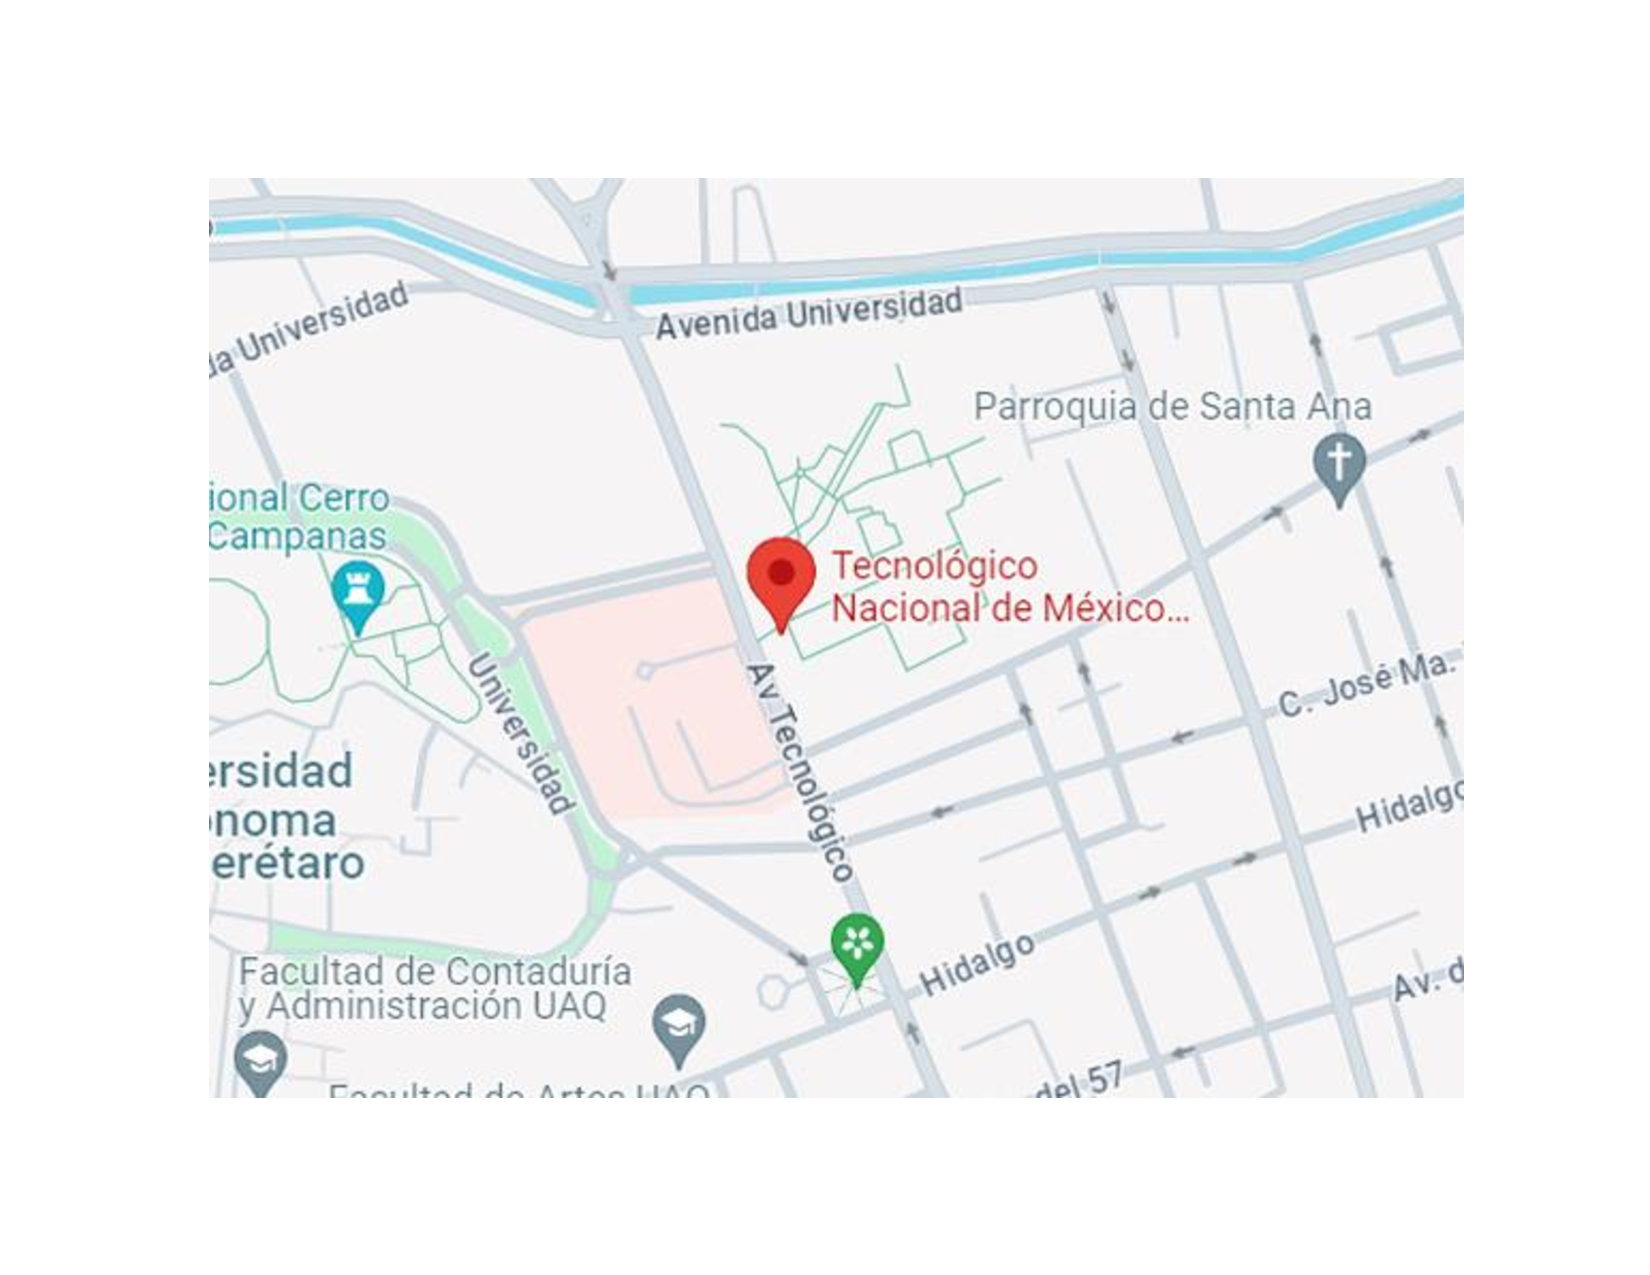
\includegraphics[scale=0.9]{14/Img/mapaItq.pdf}
        \caption{Diagrama del mapa ITQ}
        %\label{fig:mapa itq}
    \end{figure}
    % 
    % 
    
    A.1. Identificación del Riesgo
    
    Análisis detallado de la identificación de riesgos realizada durante el desarrollo del plan de emergencia. Este análisis incluye una evaluación sistemática de los riesgos internos y externos que pueden afectar la operatividad y seguridad de la industria.
    
    A.2. Riesgos Internos
    
    Descripción de algunos riesgos internos a los cuales pueden estar expuestos los alumnos. Cada riesgo se asigna un valor y una probabilidad de ocurrencia, junto con acciones preventivas.
    
    A.3. Riesgos Externos
    
    Análisis de los posibles riesgos externos que pueden ocurrir, junto con una descripción y medidas preventivas.
    
    % 
    % 
    \begin{figure}[H]
        \centering
        \includegraphics[scale=0.9]{14/Img/planoLocalización.pdf}
        \caption{Plano de Localización}
        %\label{fig:Plano Localización}
    \end{figure}
    % 
    % 
    A.4. Programa de Actividades de Prevención
    
    % 
    % 
    \begin{figure}[H]
        \centering
        \includegraphics[scale=0.9]{14/Img/EsquemaDoodle.pdf}
        \caption{Esquema Dooble}
        %\label{fig:Esquema Dooble}
    \end{figure}
    % 
    % 
    
    A.5. Plan de Acción
    
    Análisis de algunas acciones preventivas y correctivas que se pueden tomar para evitar riesgos o disminuir su probabilidad de ocurrencia.
    
    A.6. Identificación de Recursos
    
    Es crucial reconocer los recursos y herramientas disponibles durante una emergencia, conocer su ubicación y funcionamiento para prevenir negligencias y asegurar una respuesta rápida y eficiente.
    
    A.7. Identificación de Apoyos Externos
    
    A.8. Identificación de Puntos de Reunión
    
    La identificación de puntos de reunión es esencial para la seguridad durante emergencias, facilitando la comunicación y coordinación durante evacuaciones.
    
    A.9. Brigada de Evacuación
    
    A.10. Directorio de Teléfonos de Emergencia
    
    B. Determinación del Tiempo Estándar para que una Persona Competente Realice el Trabajo con Marcha Normal
    
    Visualización de diagramas manuales y Análisis MTM para determinar el tiempo Estándar.
    
    Estos son los resultados obtenidos mediante el uso del Instructivo
    \newpage
    %
    \centering{\section[\appendixautorefname{}]{Apéndice}}\label{anexo:evidencias}
    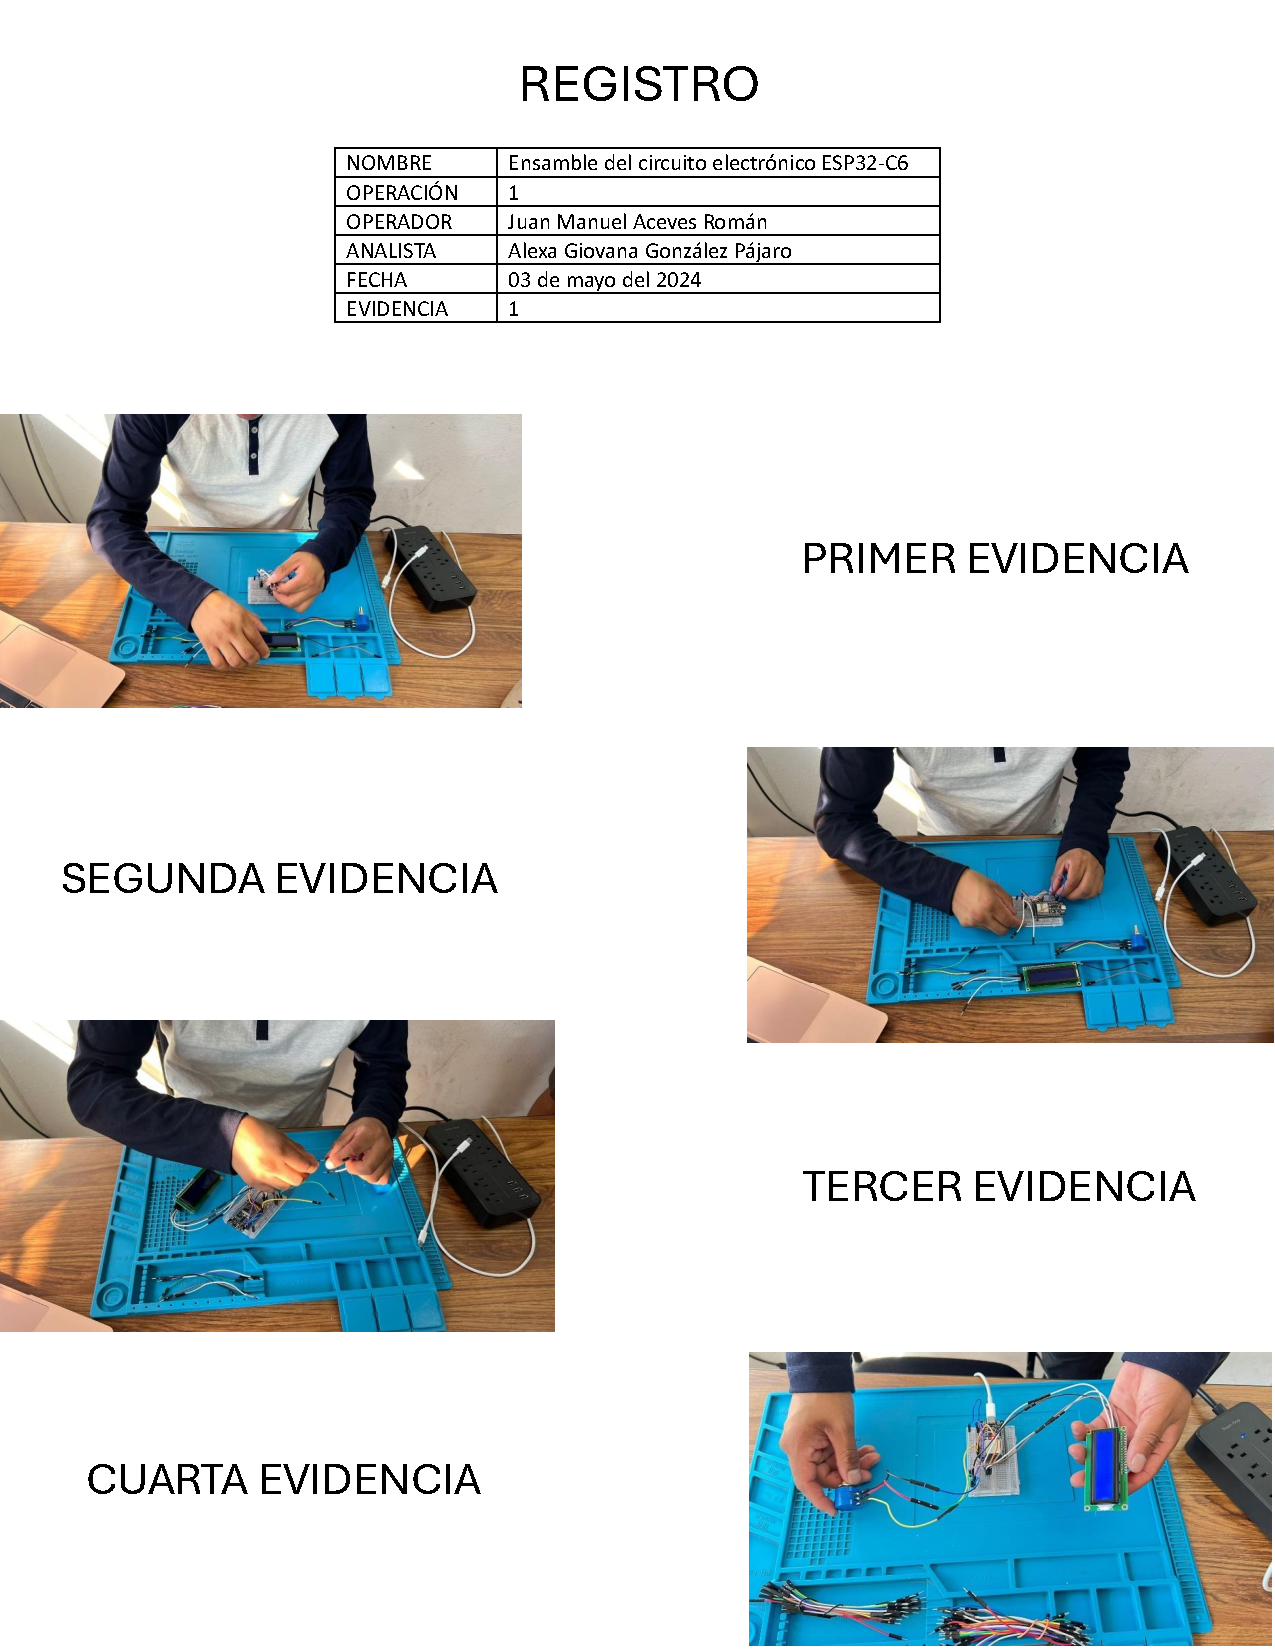
\includepdf[pages=-]{14/img/evidencias.pdf}
    
    %Antes de comenzar a preparar tu artículo, es importante que lea primero la guía del autor, la cual incluye los temas o apartados que son necesarios para tener tu trabajo completo.
    %Una vez completada la edición del texto, el documento está listo para el uso de esta plantilla. En este archivo recién creado, resalte todo el contenido e importe el archivo de texto preparado. Ahora esta listo para estilizar su documento.
    %En esta sección se deben presentar todo lo obtenido de la sección 2, incluidas deducciones o efectos del desarrollo. También se podrán incluir subsecciones numeradas de la siguiente forma:
    
    \subsection{Autores y Afiliaciones}
    
    Para distinguir las afiliaciones de los autores, utilice superíndices iniciando con el número 1, 2, etc., sucesivamente, esto dependerá de la cantidad de los departamentos a los que estén afiliados los autores. En caso de que todos los autores pertenezcan a una mismo departamento e institución, utilizar sólo el superíndice 1. 
    
    \subsection{Identificar los encabezados}
    
    Se les recuerda a los autores que los encabezados deben de estar conforme los solicita la guía del autor. De ahí se puede adaptar el trabajo para que sea más fácil de entender para el lector.
    Los encabezados organizan los temas sobre una base relacional y jerárquica. Por ejemplo, el título del documento es encabezado del texto principal porque todo el material posterior se relaciona y elabora sobre este tema. 
    
    \subsection{Tablas y Figuras}
    \newpage
    %
    \centering{\section[\appendixautorefname{}]{Apéndice}}\label{anexo:Tiempos}
    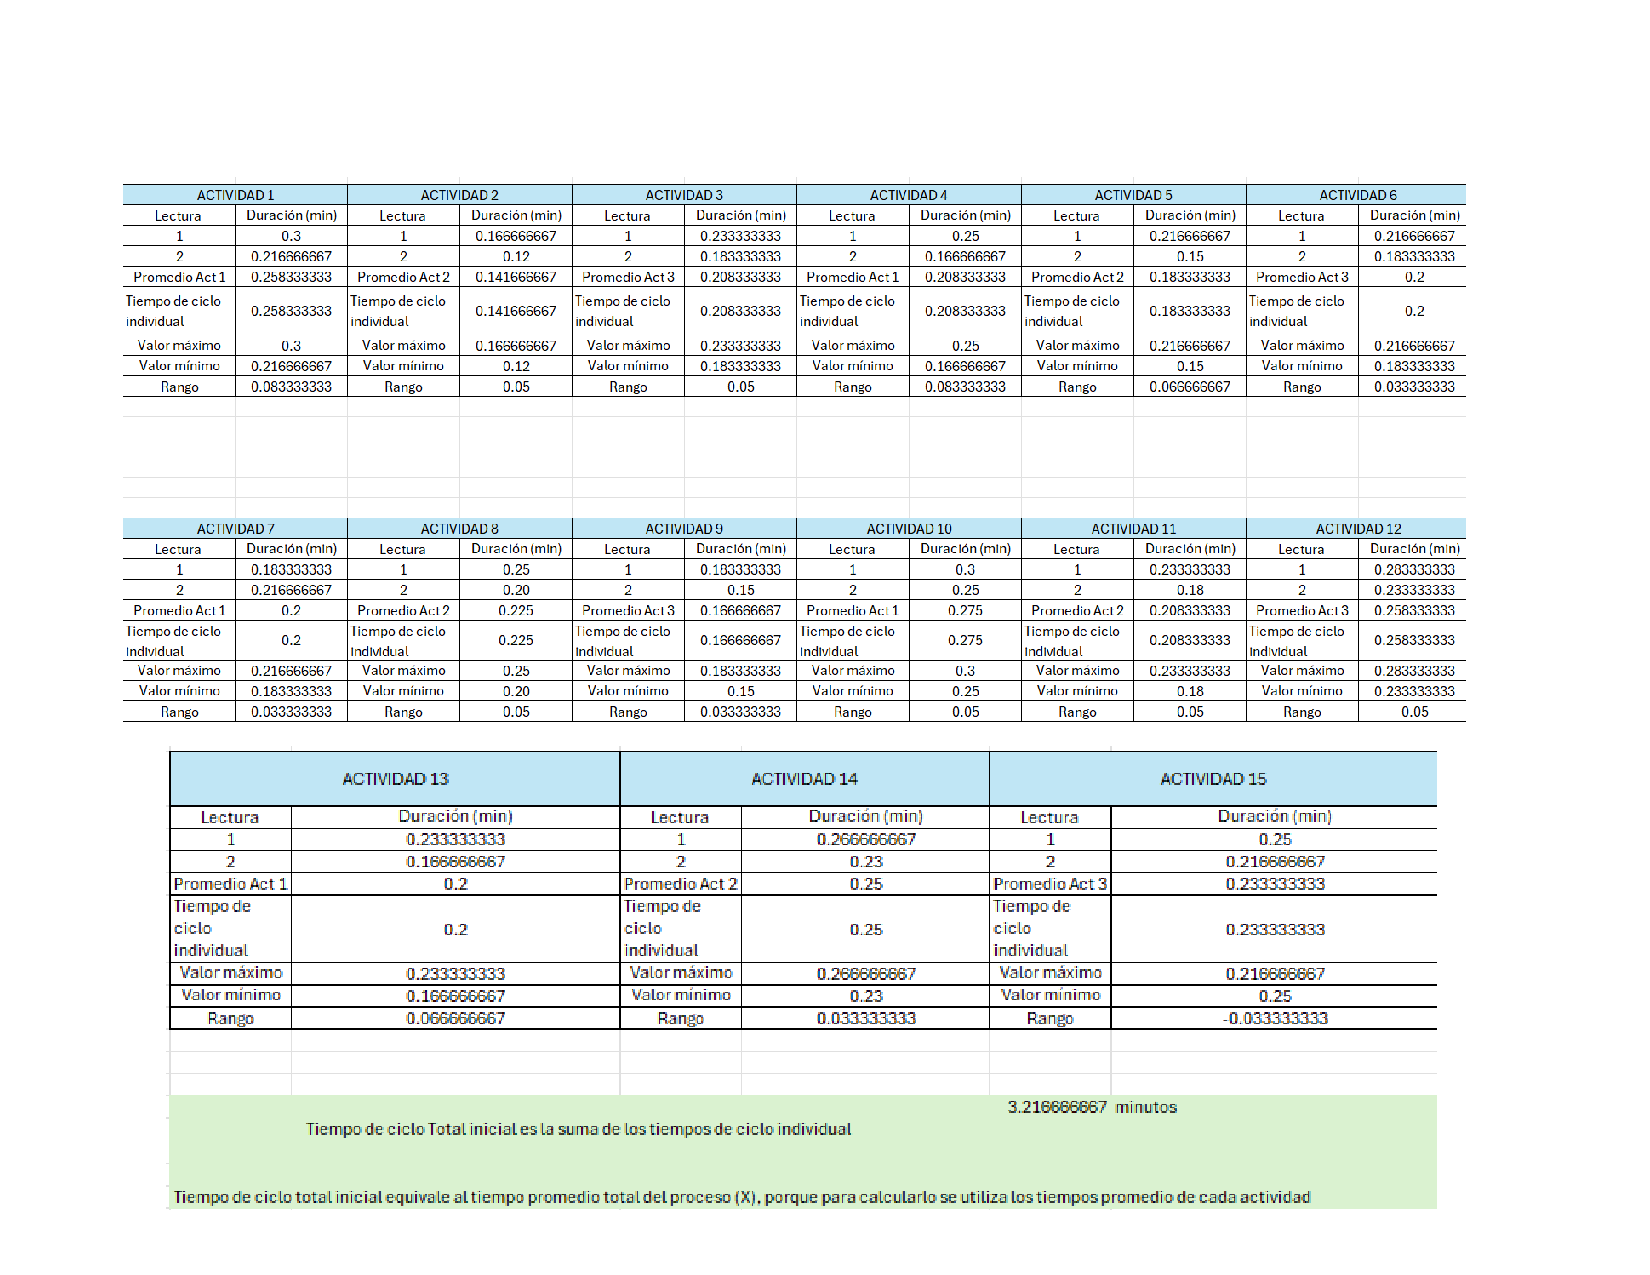
\includepdf[pages=-]{14/img/Tiempos.pdf}
    \begin{enumerate}
        \item Posición de las tablas y figuras: Coloque las figuras y las tablas en la parte superior e inferior de las columnas. Evite colocarlos en medio. Las figuras y las tablas grandes pueden abarcar ambas columnas. Los títulos de las figuras deben de estar debajo de las mismas; los títulos de las tablas deben aparecer encima de ellas. Insértese las figuras y los cuadros después de citarse en el texto. Utilice la abreviatura “Fig. 1”, incluso al principio de una oración. 
    \end{enumerate}
    
    \section{Conclusiones}
    
        Se estableció el objetivo de buscar la manera más económica de realizar el trabajo a través de un circuito electrónico, realizando un estudio de tiempos y movimientos. A pesar de las dificultades técnicas con algunos materiales, se comprobó la hipótesis de que mediante un buen análisis de tiempos y movimientos, eliminando movimientos innecesarios, modificando materiales y aplicando metodologías como las 5S, se pueden reducir tiempos y aumentar la productividad, resultando en la reducción de costos.
    
    
    %Se describe aquí el alcance del trabajo, logros obtenidos y perspectivas para el futuro de este. Se sugiere colocar información cuantitativa obtenida.
    
    \section{Agradecimientos}
    
    Es importante darles su debido reconocimiento a los laboratorios, instituciones, organizaciones, entre otros que han sido participes para la culminación de este trabajo. También es importante mencionar, fondos, proyectos, becas, entre otros que se le han otorgado al o los autores para realizar el trabajo de investigación. Ejemplo: “Los autores agradecen al Concejo Nacional de Ciencia y Tecnología por los recursos otorgados…”
    
    \section*{Referencias}
    
    %Para esta platilla, se solicita al autor enumerar las citas de manera consecutiva entre corchetes \cite{YLi2013}. 
    %La puntuación de la oración que sigues sería \cite{Mesaelides2011}. 
    %Refiérase simplemente al número de referencia, como en \cite{Morales2012}, no utilice “Ref. [3]” o “referencia [3]” excepto al principio de una oración: “La referencia [3] fue la primera…”
    Enumere las notas al pie por separado en superíndices. Coloque la nota de pie de en la parte inferior de la columna en la que se citó. No coloque notas al pie en la lista de referencias. Utilice letras para las notas al pie de la tabla.
    A menos de que haya tres autores o más; no utilice “et al.”. Los trabajos que no hayan sido publicados, incluso si han sido presentados para su publicación, deben ser citados como “inéditos”. Los trabajos que han sido aceptados para su publicación deben de citarse como “en prensa”. Poner en mayúscula sólo la primera palabra de un título, excepto los nombres propios y los símbolos de elemento. 
    %Otros ejemplos \cite{LAAngeles2021}, \cite{LAAngelesConni}. 
    %Véase el link \cite{prueba}, Véase el Apéndice \ref{anexo:pines}.
    
    % Ejemplo
    %  @Article{article,
    % 	author = "Author1 LastName1 and Author2 LastName2 and Author3 LastName3",
    % 	title = "Article Title",
    % 	volume = "30",
    % 	number = "30",
    % 	pages = "10127-10134",
    % 	year = "2013",
    % 	doi = "10.3389/fnins.2013.12345",
    % 	URL = "http://www.frontiersin.org/Journal/10.3389/fnins.2013.12345/abstract",
    % 	journal = "Frontiers in Neuroscience"
    % }
    
    % @book{book,
    %   author    = {Author Name}, 
    %   title     = {The title of the work},
    %   publisher = {The name of the publisher},
    %   address   = {The city},
    %   year      = 1993,
    % }
    
    % @incollection{chapter,
    %   author       = {Bauthor Surname}, 
    %   title        = {The title of the work},
    %   editor       = {Editor Name},
    %   booktitle    = {The title of the book},
    %   publisher    = {The name of the publisher},
    %   address      = {The city},
    %   year         = 2002,
    %   pages        = {201-213},
    % }
    
    % @InProceedings{conference,
    %   author = {Cauthor Name and Dauthor Surname and Fauthor LastName},
    %   title = {The title of the work},
    %   booktitle = {The title of the conference proceedings},
    %   year = 1996,
    %   publisher = {The name of the publisher},
    %   editor = {Editor Name1 and Editor Name2},
    %   pages = {41-50},
    % }
    
    % @book{cho,
    %   author       = {Gauthor Name1}, 
    %   title        = {The title of the work},
    %   publisher = {Country code and patent number},
    %   address      = {Patent Country},
    %   year = 2013
    % }
    
    % @book{patent,
    %   author    = {Hauthor Surname1}, 
    %   title     = {The title of the work},
    %   publisher = {Patent number},
    %   address   = {Patent country},
    %   year      = 2010,
    % }
    
    % % please use misc for datasets
    % @misc{dataset, 
    % 	author = "Author1 LastName1 and Author2 LastName2 and Author3 LastName3",
    % 	title = "Data Title",
    % 	year = "2011",
    % 	doi = "10.000/55555",
    % 	URL = "http://www.frontiersin.org/",
    % }
    
    \bibliographystyle{ieeetr}
    \bibliography{14/referencias}
    % 
    % 
    %%%%%%%%%%%%%%%%%%%%%%%%%%%%%%%%%%
    \appendix
    %%%%%%%%%%%%%%%%%%%%%%%%%%%%%%%%%%
    % 
    % 
    \newpage
    \centering{\section[\appendixautorefname{}]{Apéndice}}\label{anexo:cables}
    \includepdf[pages=-]{14/img/cables de conexión .pdf}
    %
    \centering{\section[\appendixautorefname{}]{Apéndice}}\label{anexo:ESP32-C6}
    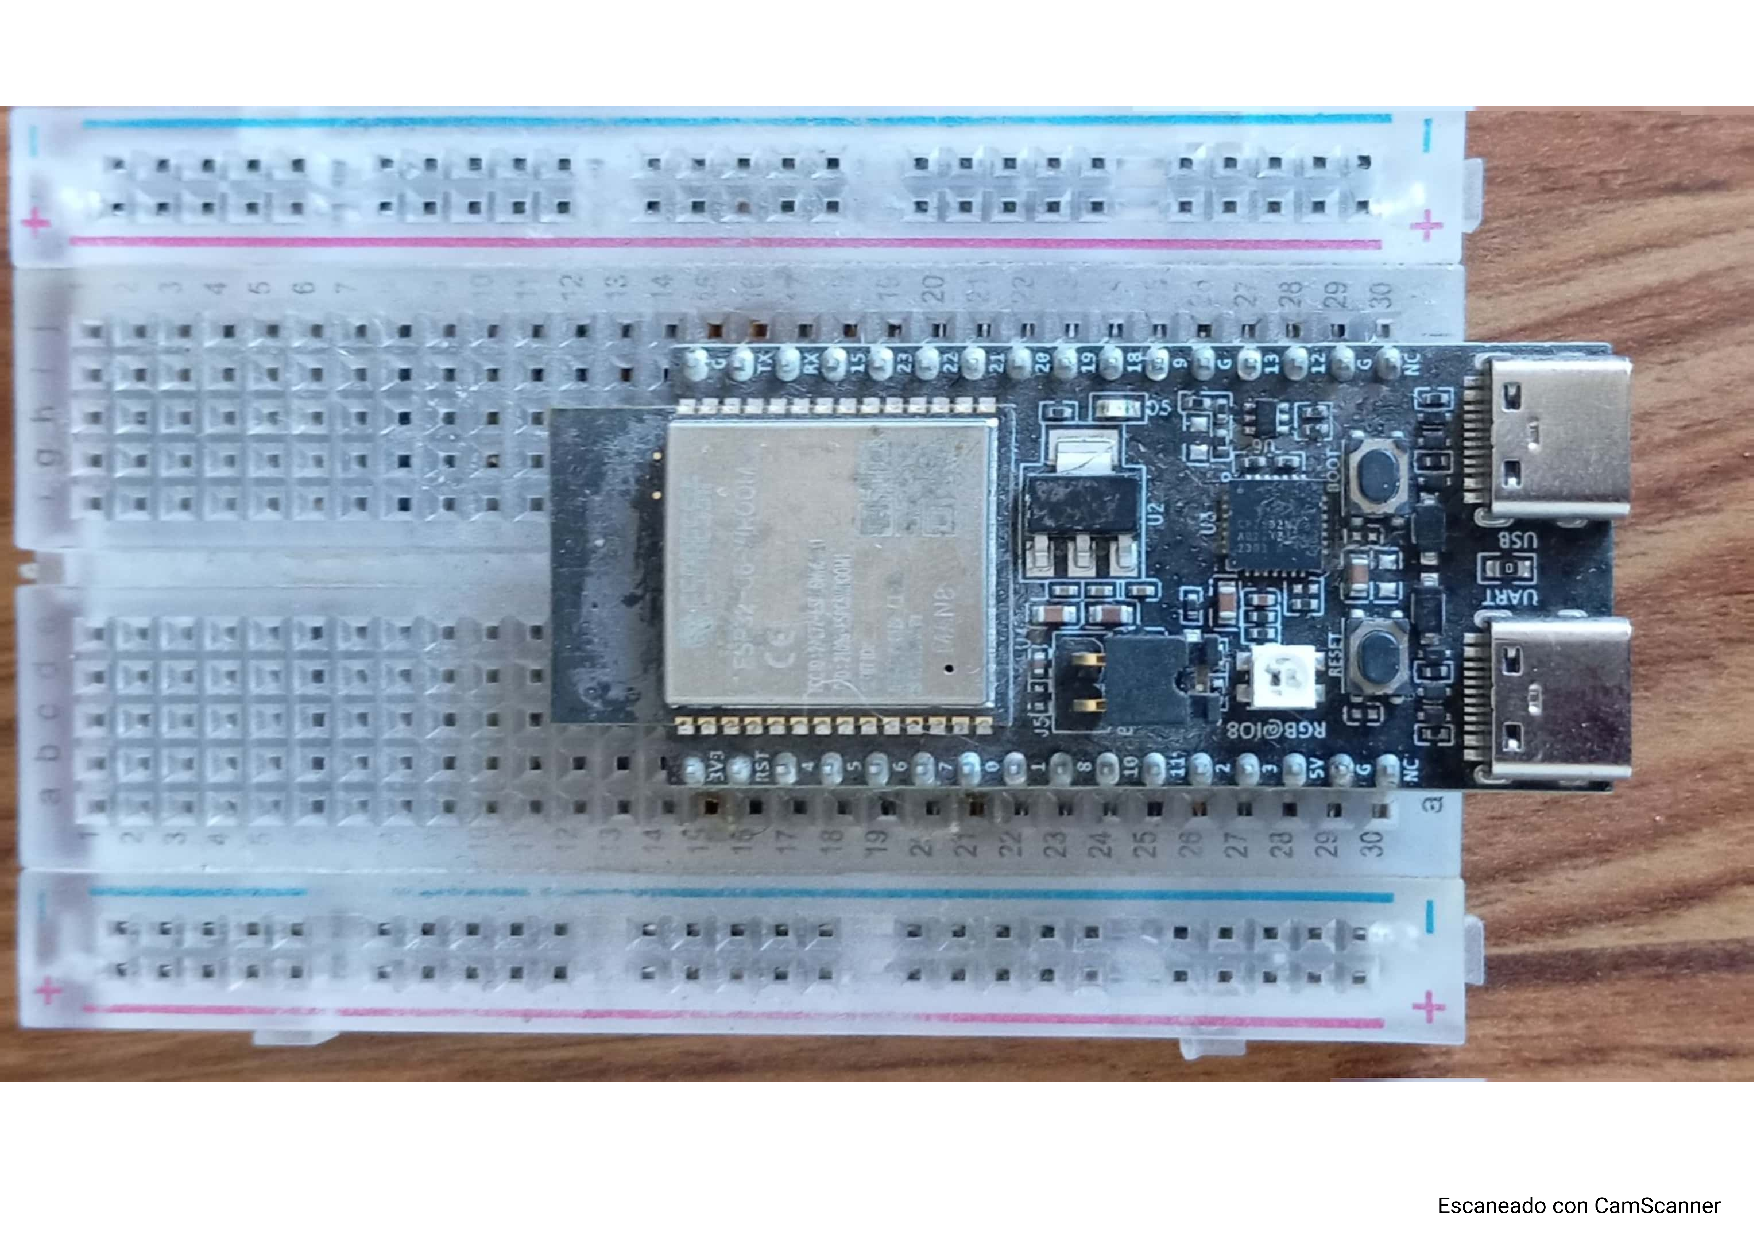
\includepdf[pages=-]{14/img/ESP32-C6.PDF}
    %
    \centering{\section[\appendixautorefname{}]{Apéndice}}\label{anexo:LCD 16x2}
    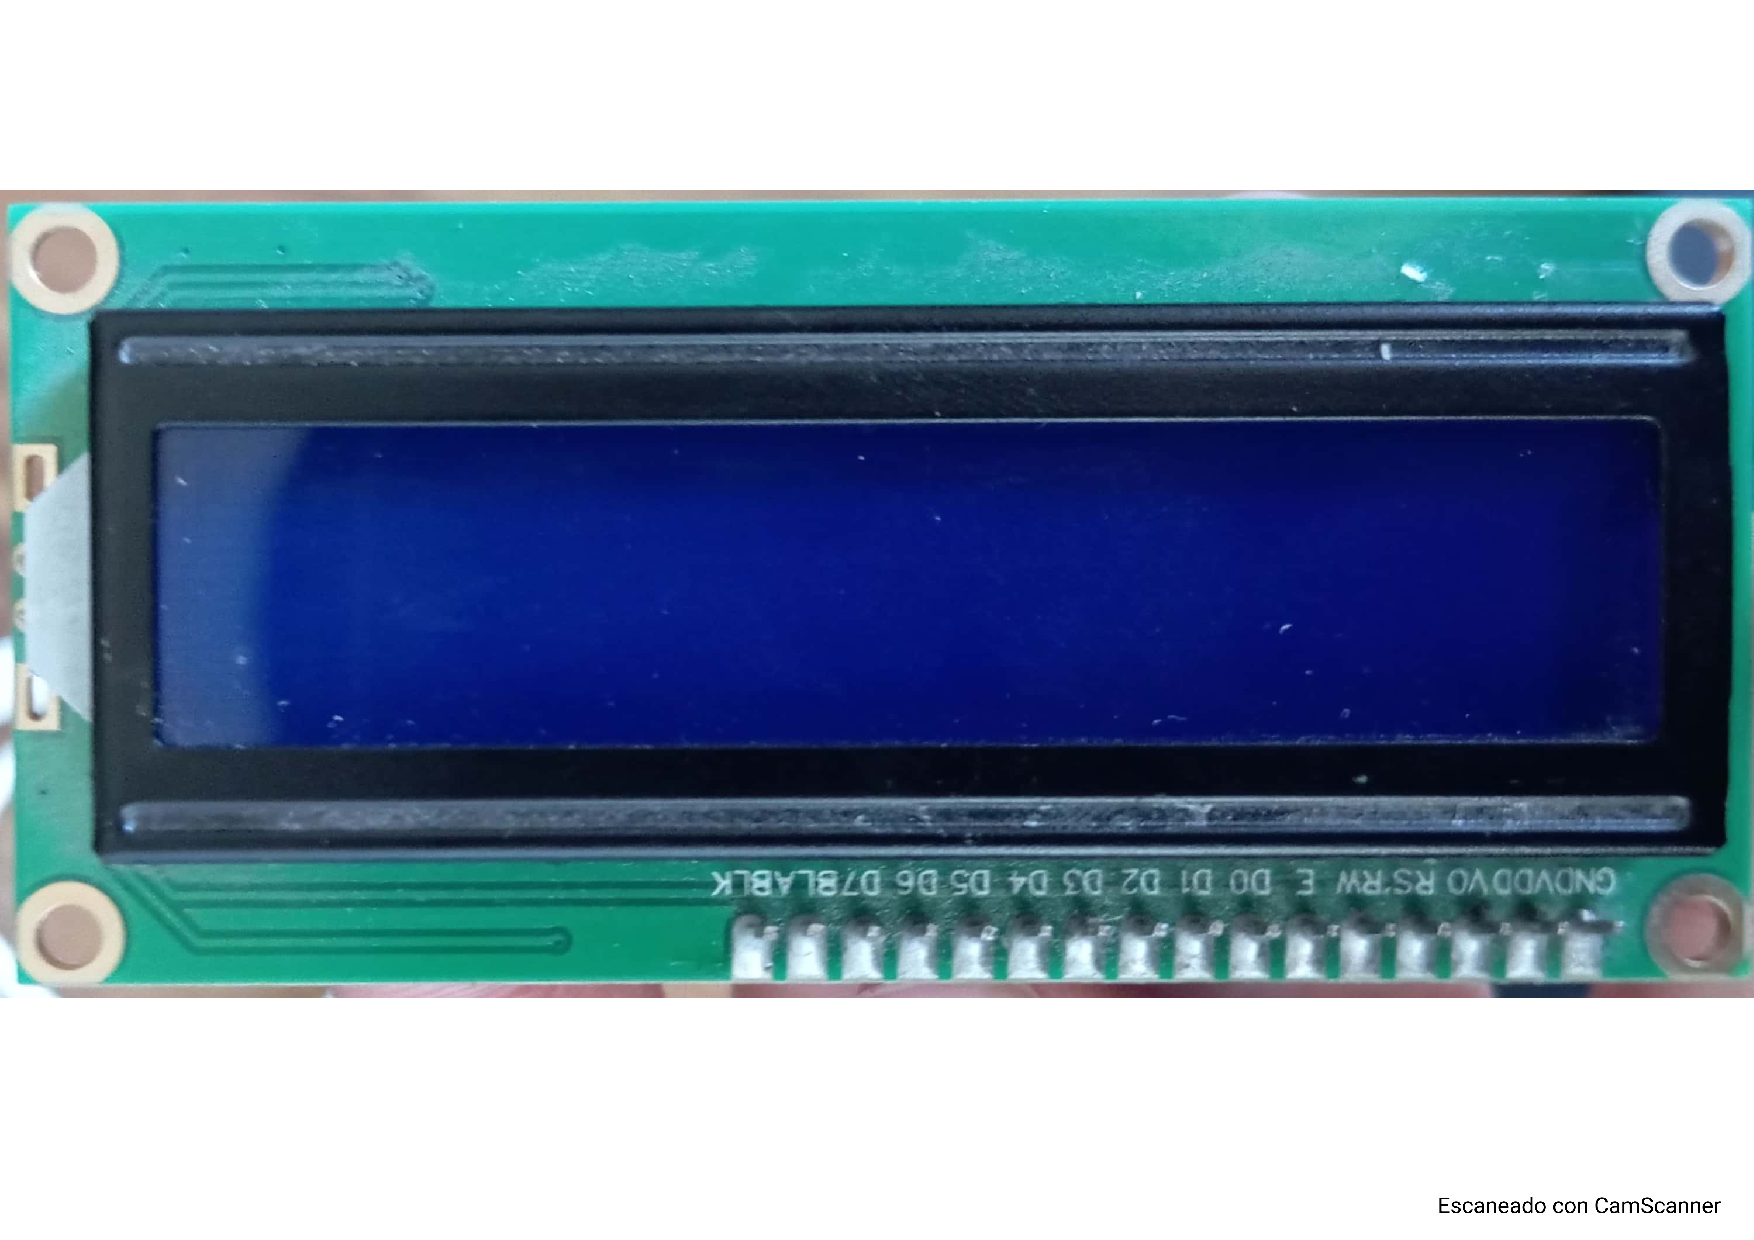
\includepdf[pages=-]{14/img/LCD 16x2.pdf}
    %
    \centering{\section[\appendixautorefname{}]{Apéndice}}\label{anexo:multicontanto}
    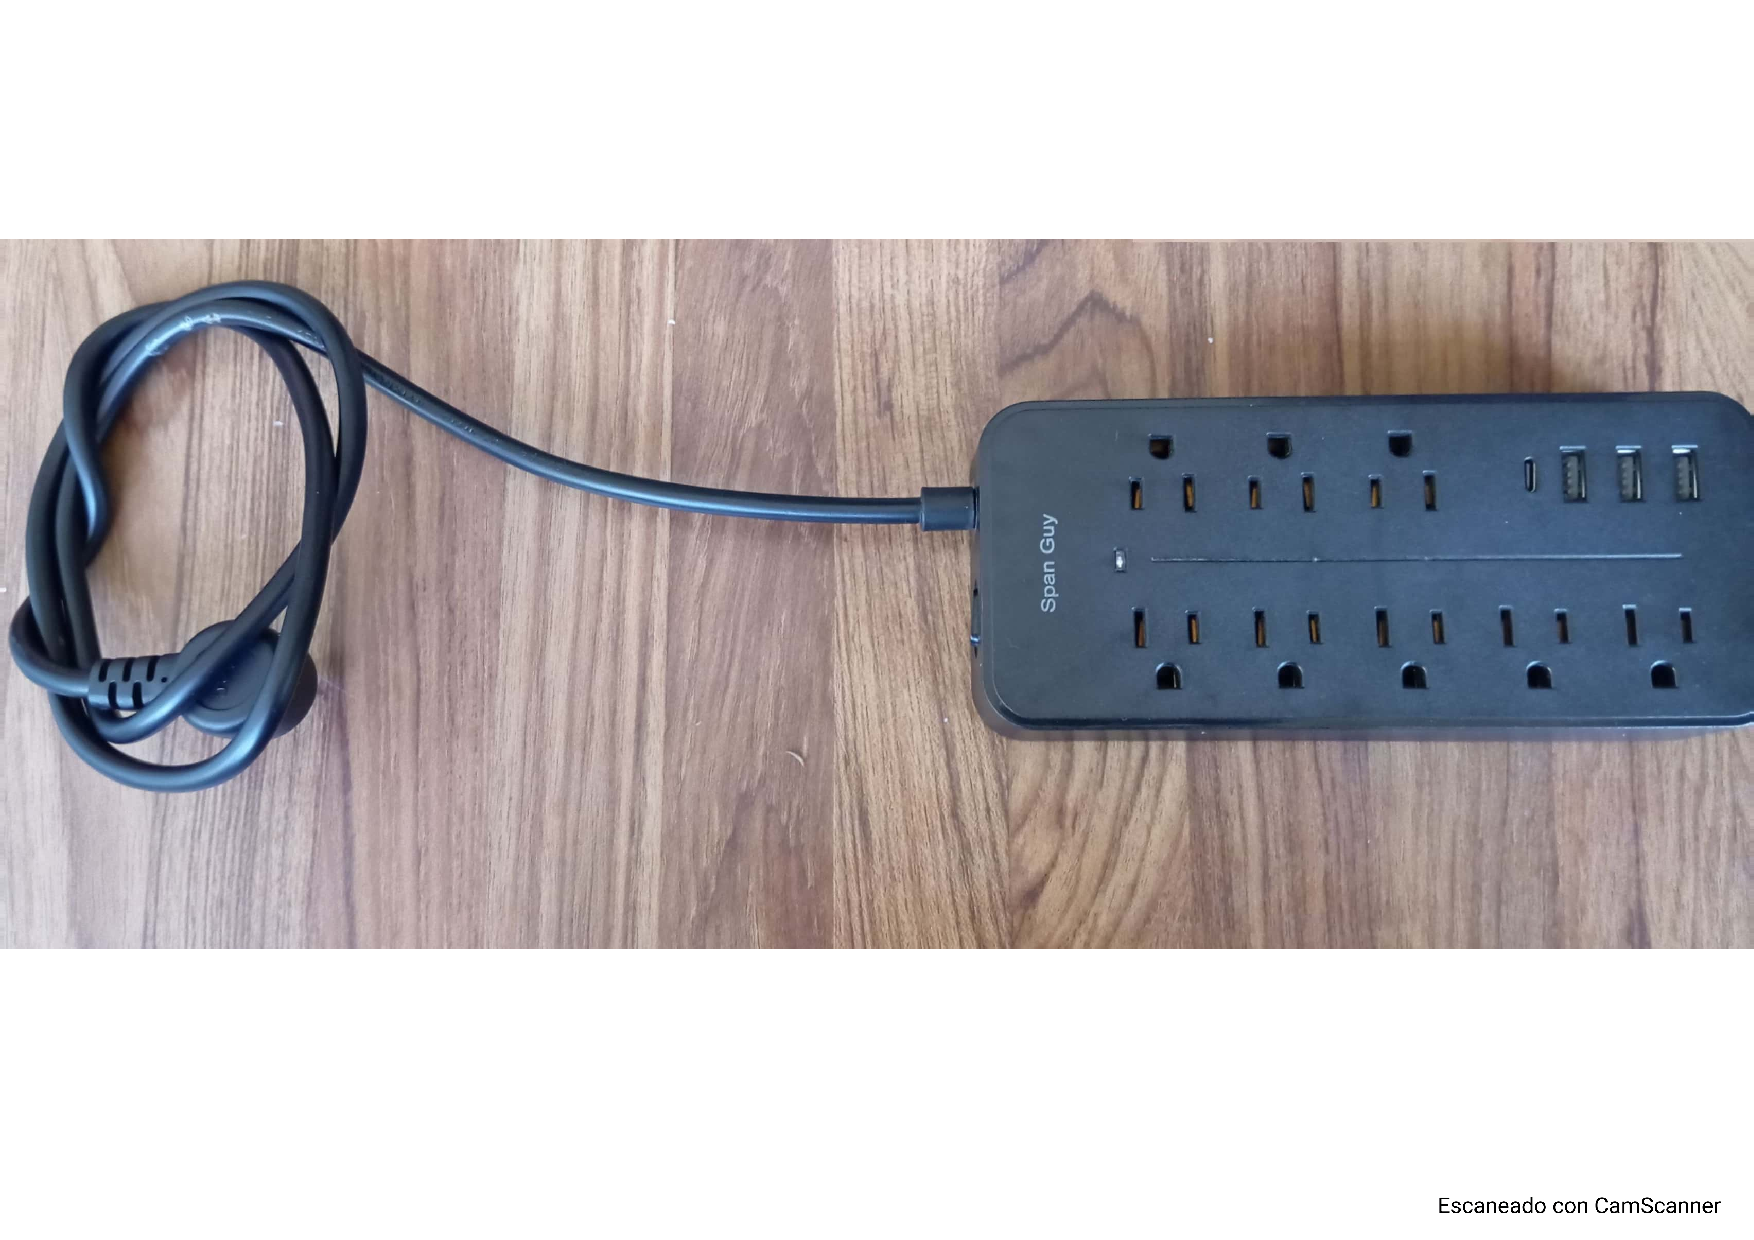
\includepdf[pages=-]{14/img/multicontanto.pdf}
    %
    \centering{\section[\appendixautorefname{}]{Apéndice}}\label{anexo:resistencia}
    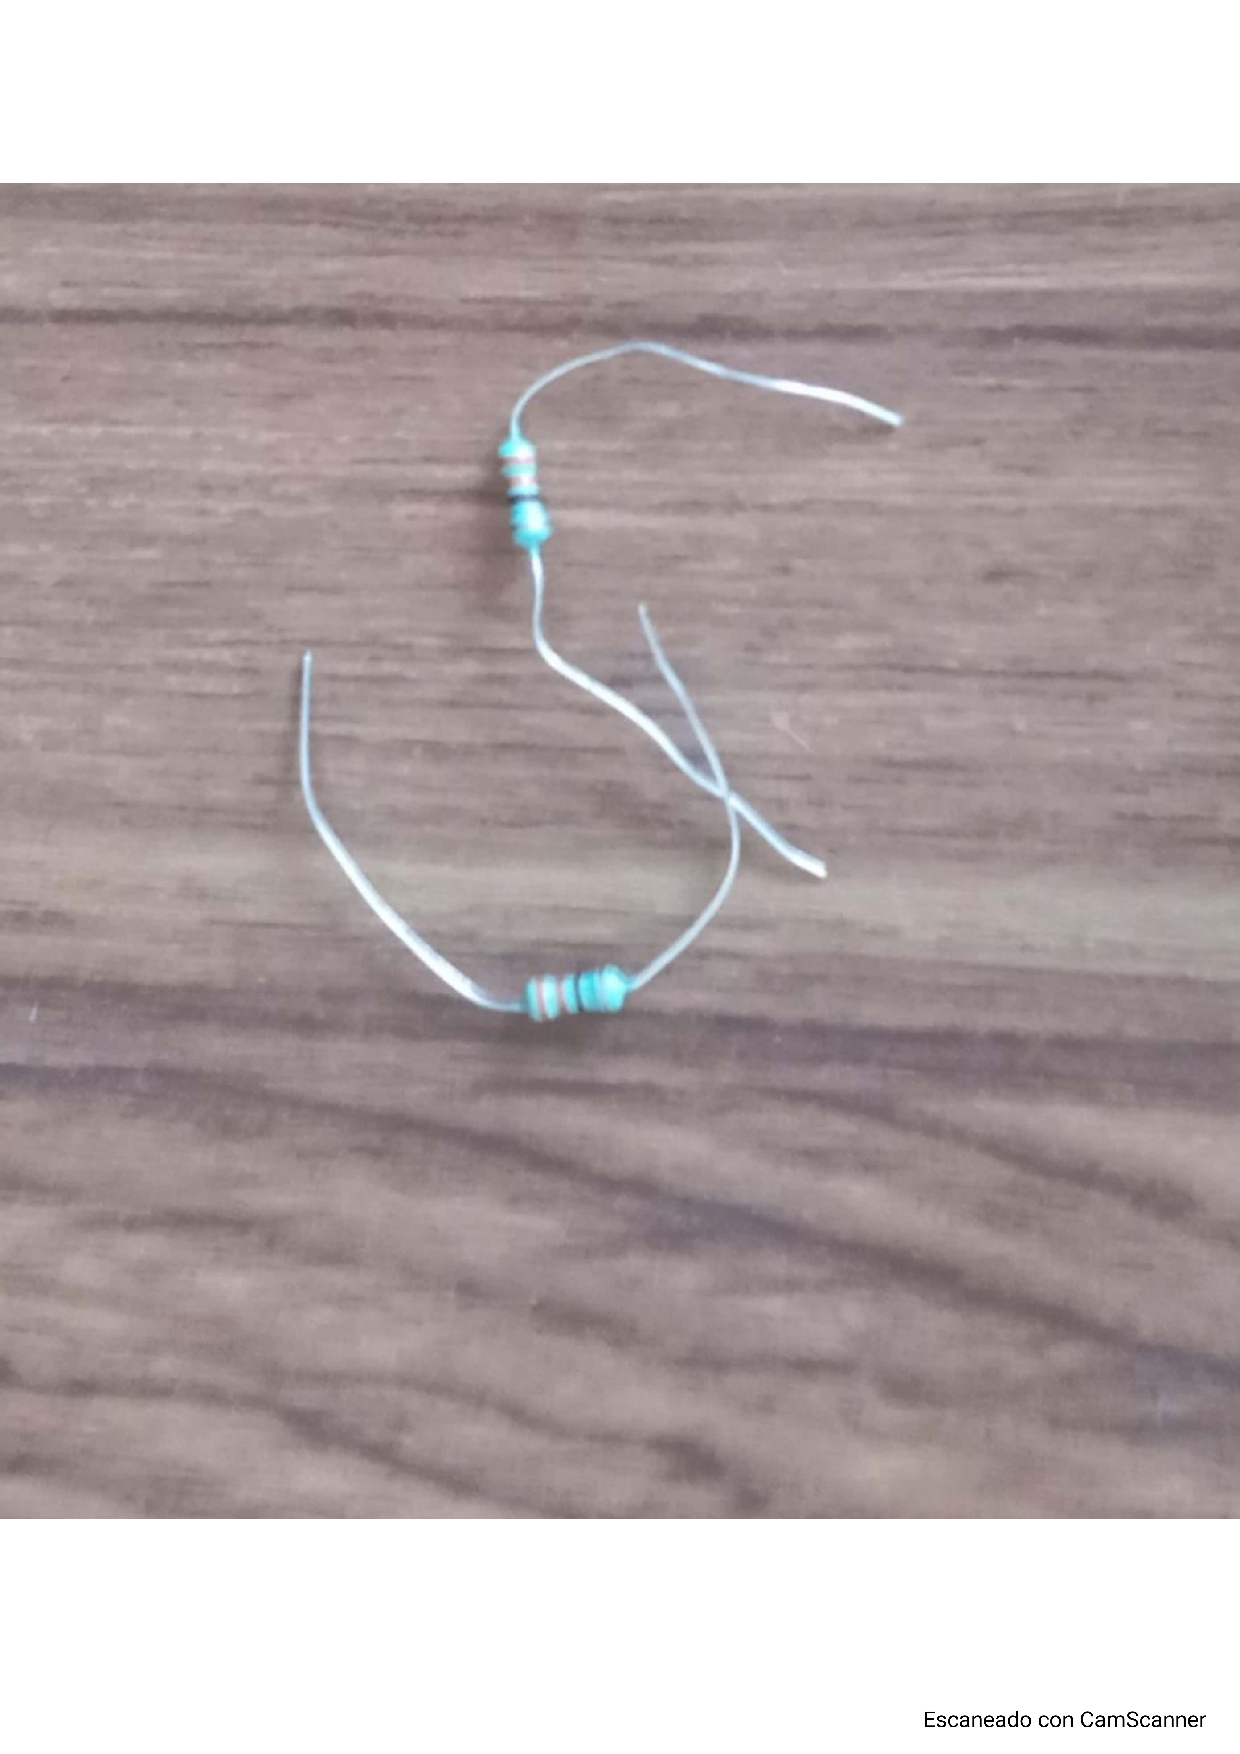
\includepdf[pages=-]{14/img/resistencia.pdf}
    %
    \centering{\section[\appendixautorefname{}]{Apéndice}}\label{anexo:Instructivo}
    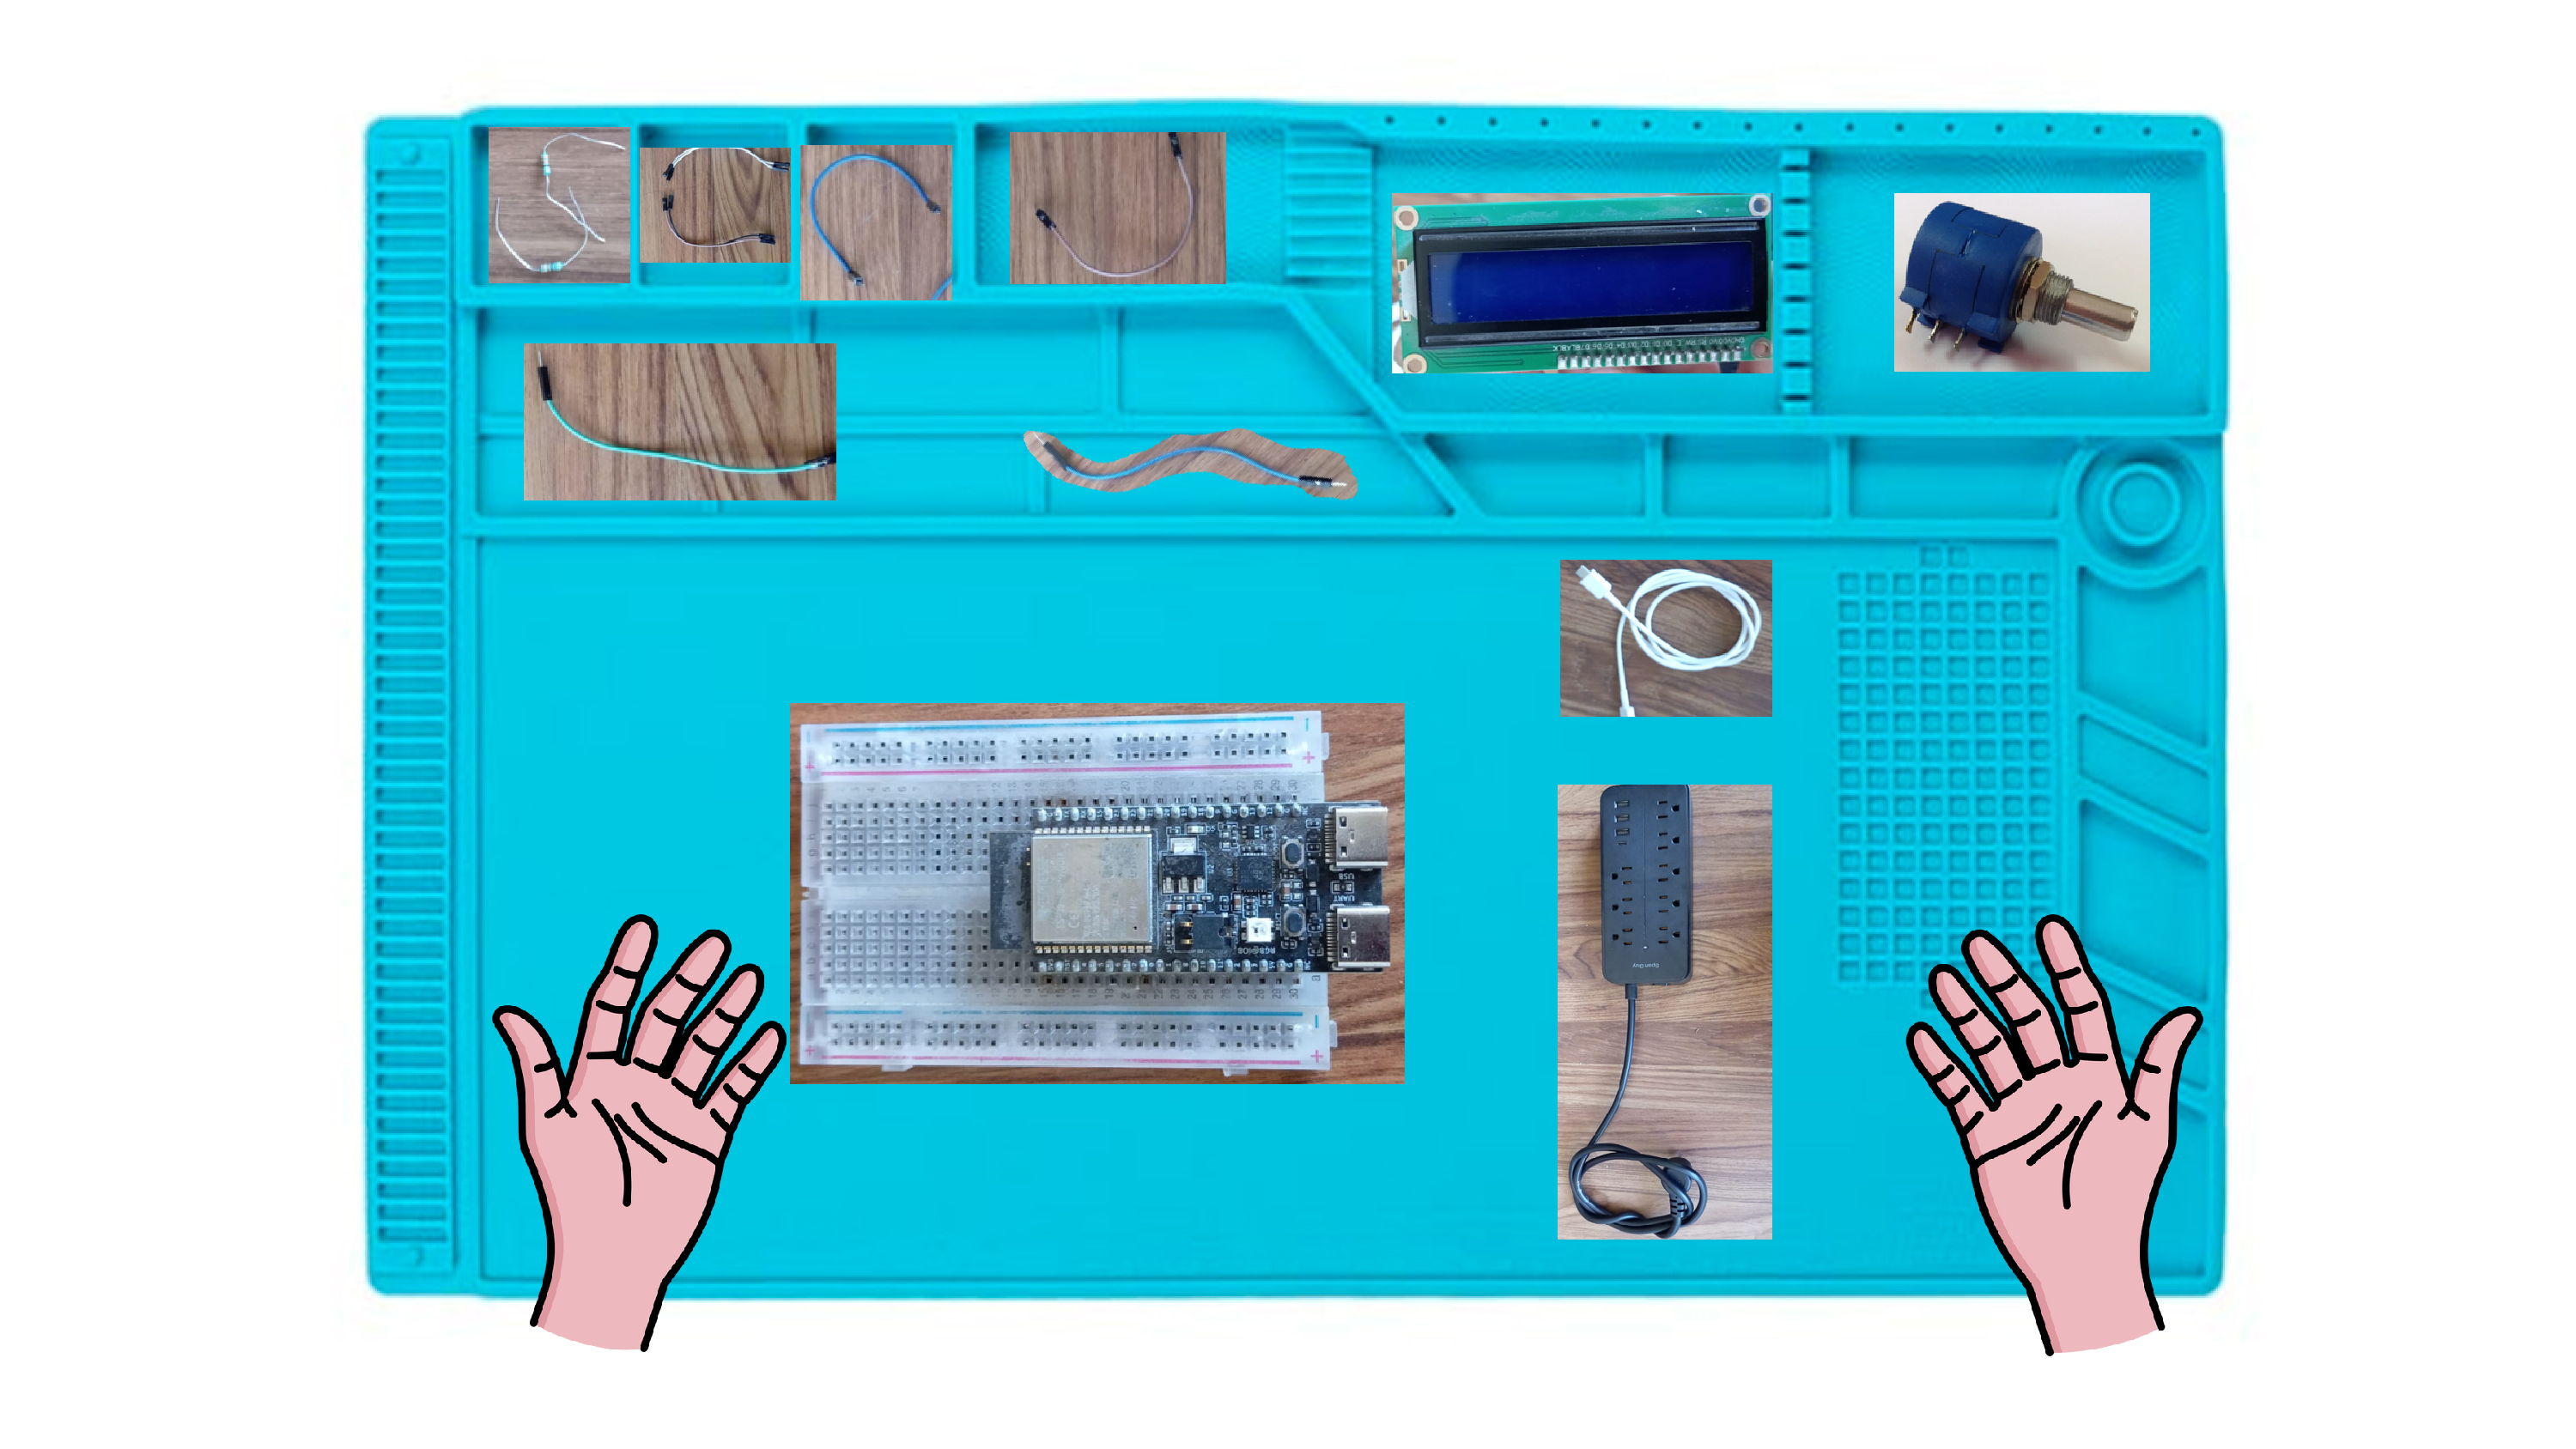
\includepdf[pages=-]{14/img/Instructivo.pdf}
    %
    \centering{\section[\appendixautorefname{}]{Apéndice}}\label{anexo:PlanoCableMh}
    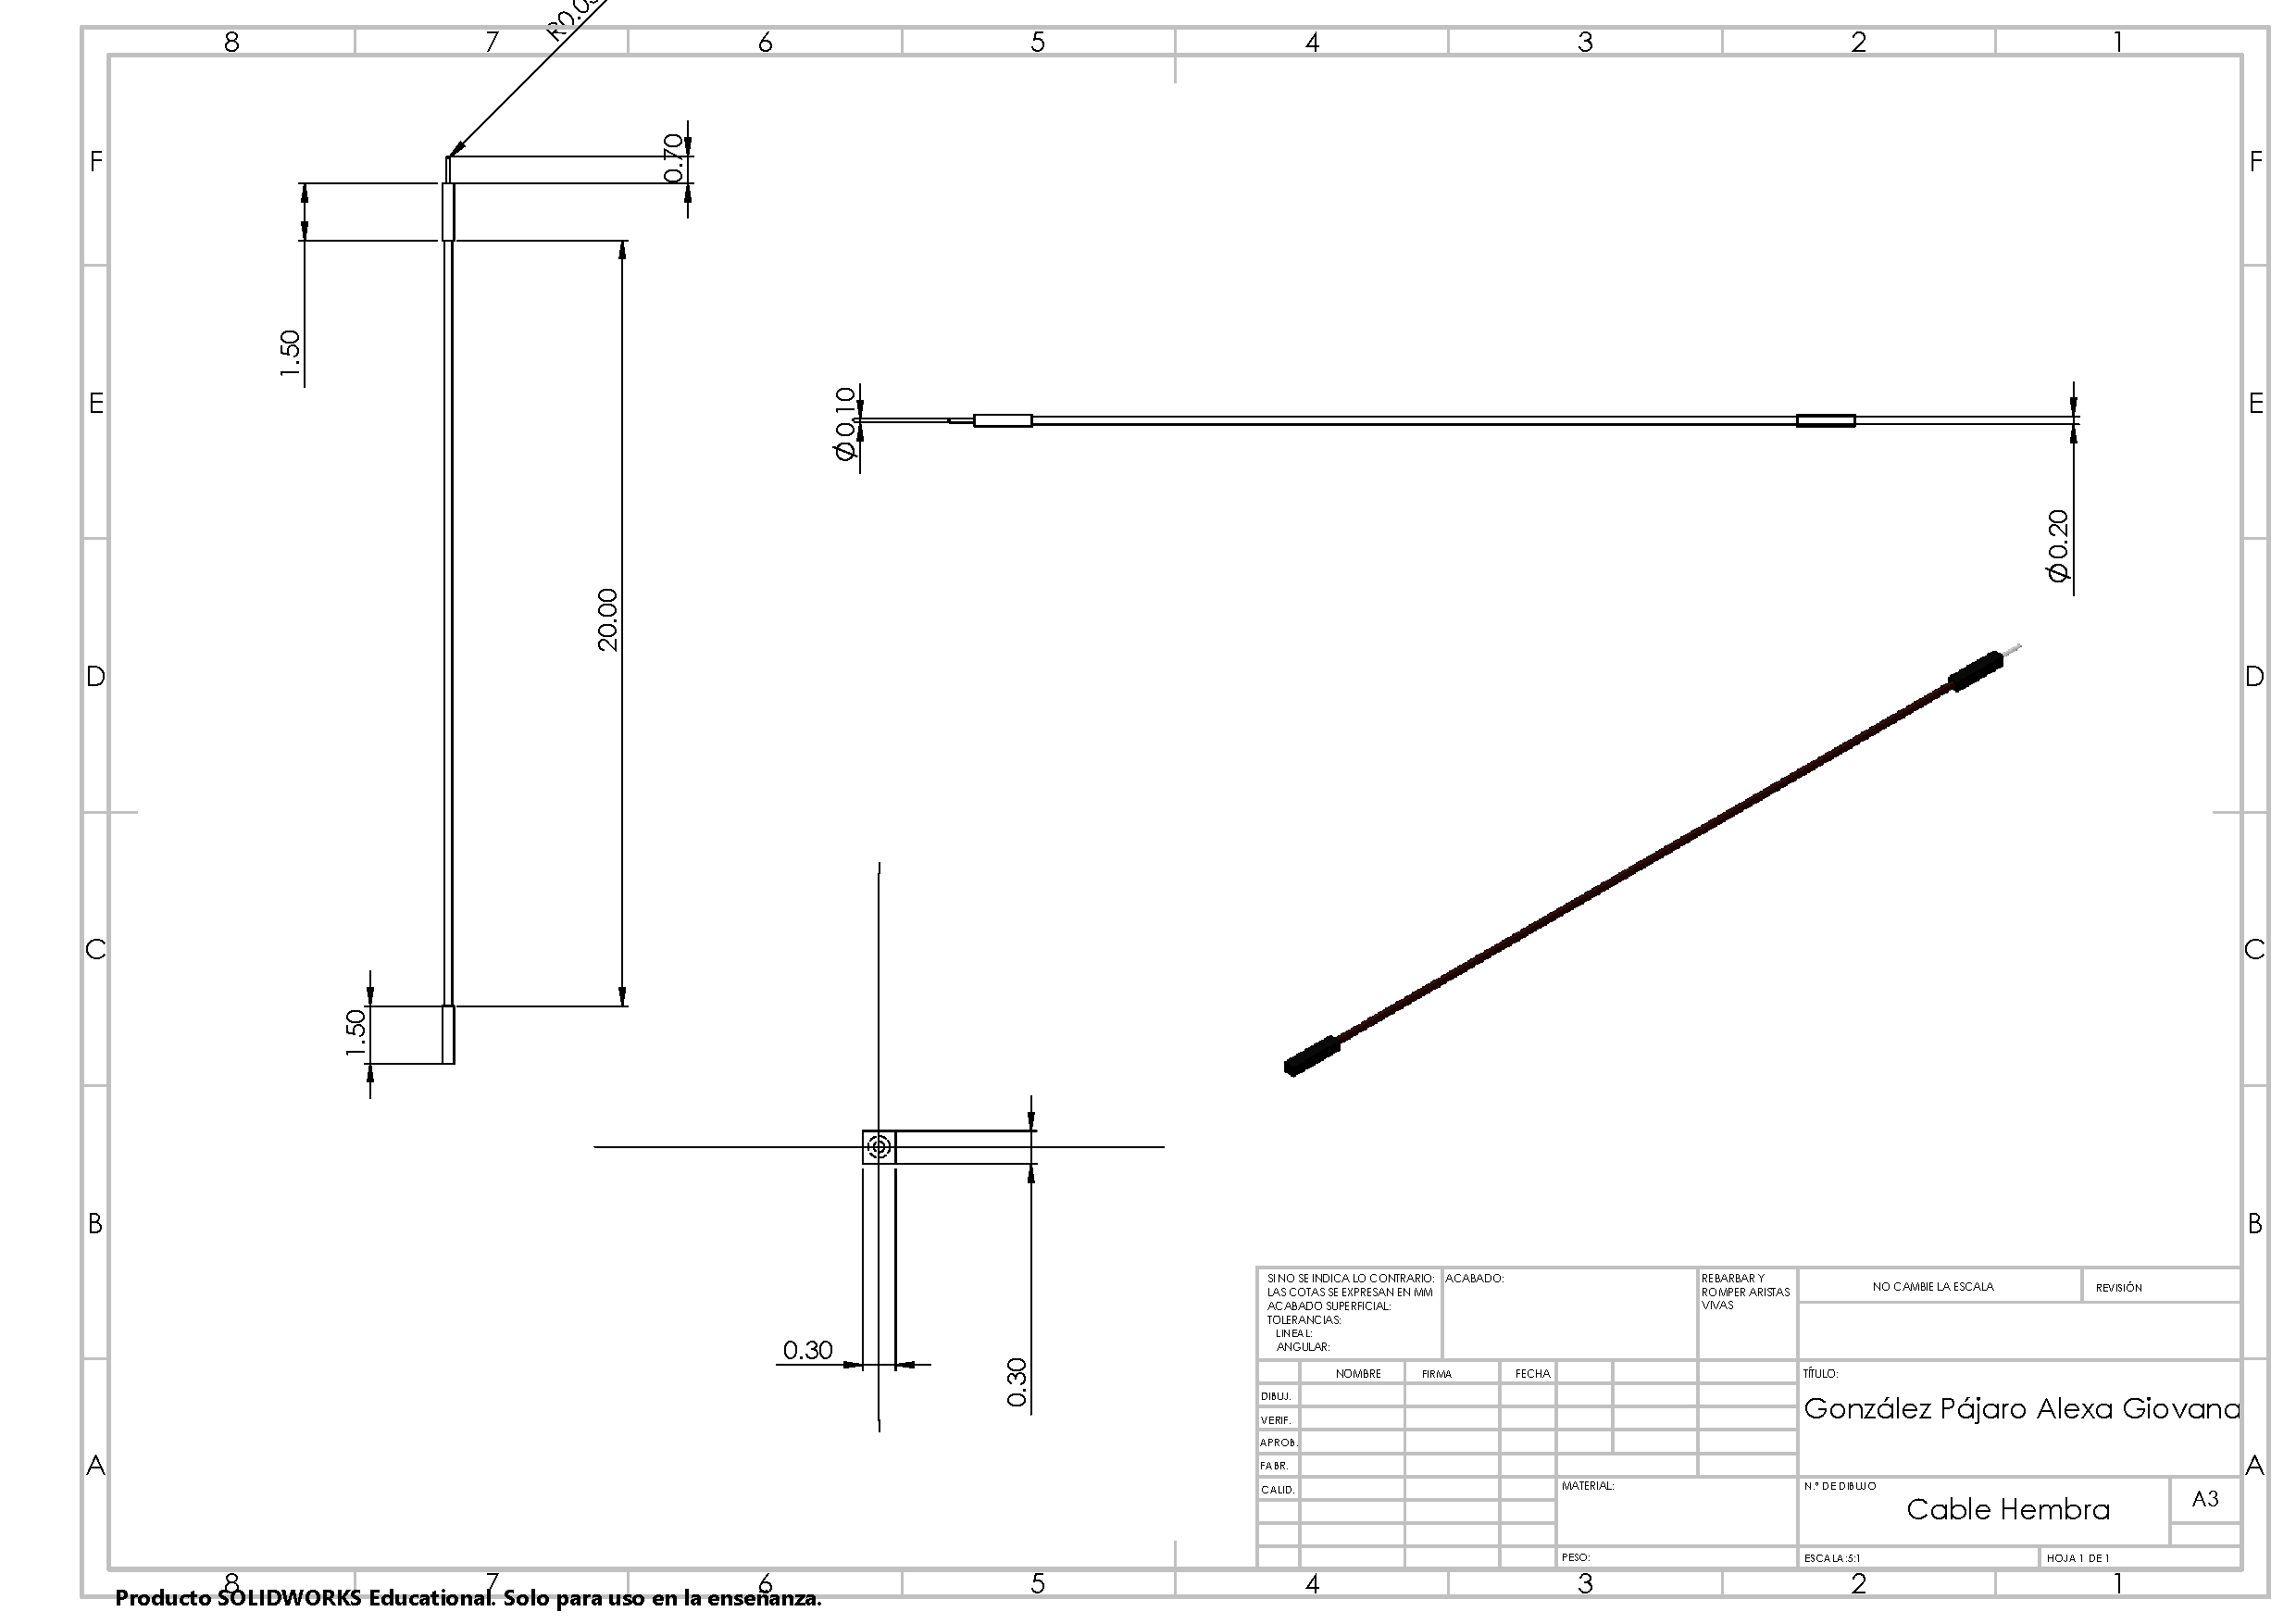
\includepdf[pages=-]{14/img/PlanoCableMh.pdf}
    %
    \centering{\section[\appendixautorefname{}]{Apéndice}}\label{anexo:PlanoCableMm}
    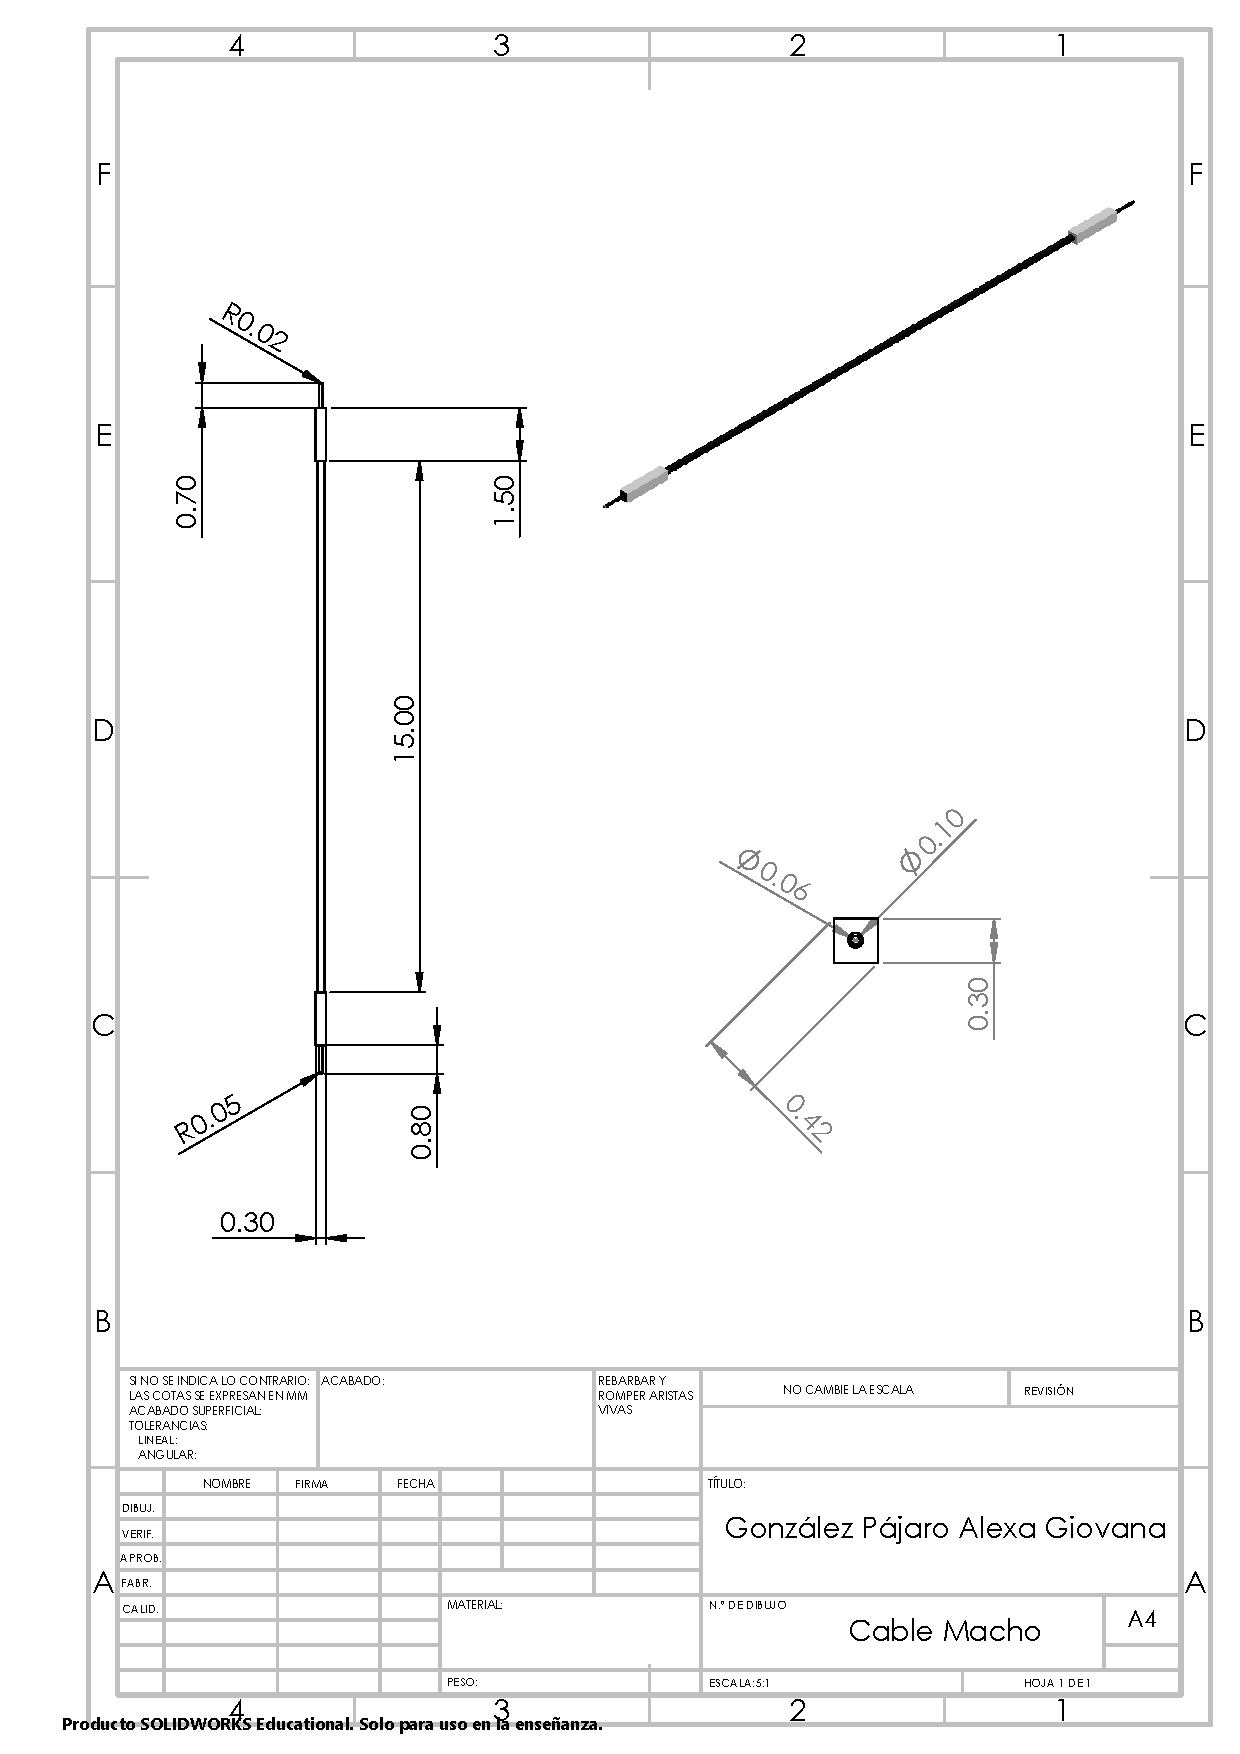
\includepdf[pages=-]{14/img/PlanoCableMm.PDF}
    %
    \centering{\section[\appendixautorefname{}]{Apéndice}}\label{anexo:PlanoLcd}
    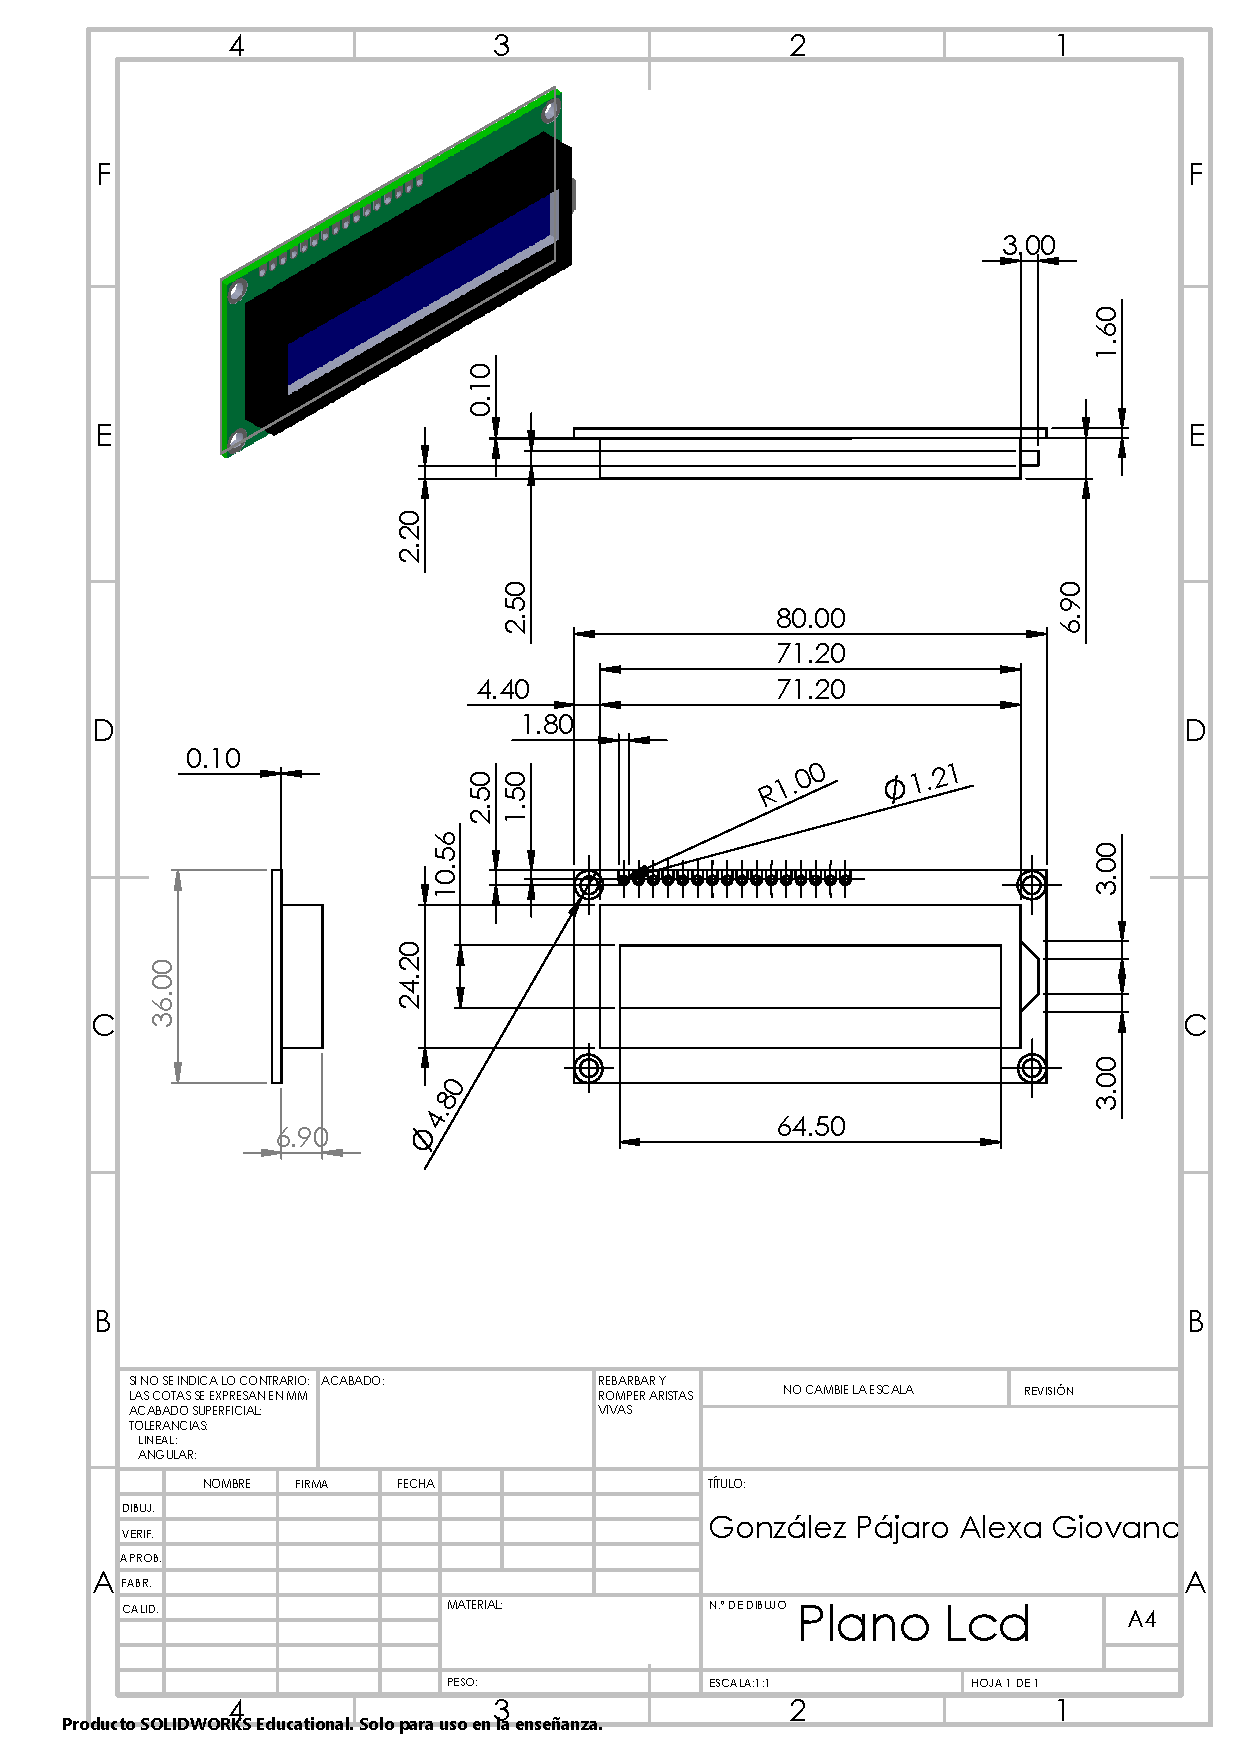
\includepdf[pages=-]{14/img/PlanoLcd.pdf}
    %
    \centering{\section[\appendixautorefname{}]{Apéndice}}\label{anexo:PlanoPotenciometro}
    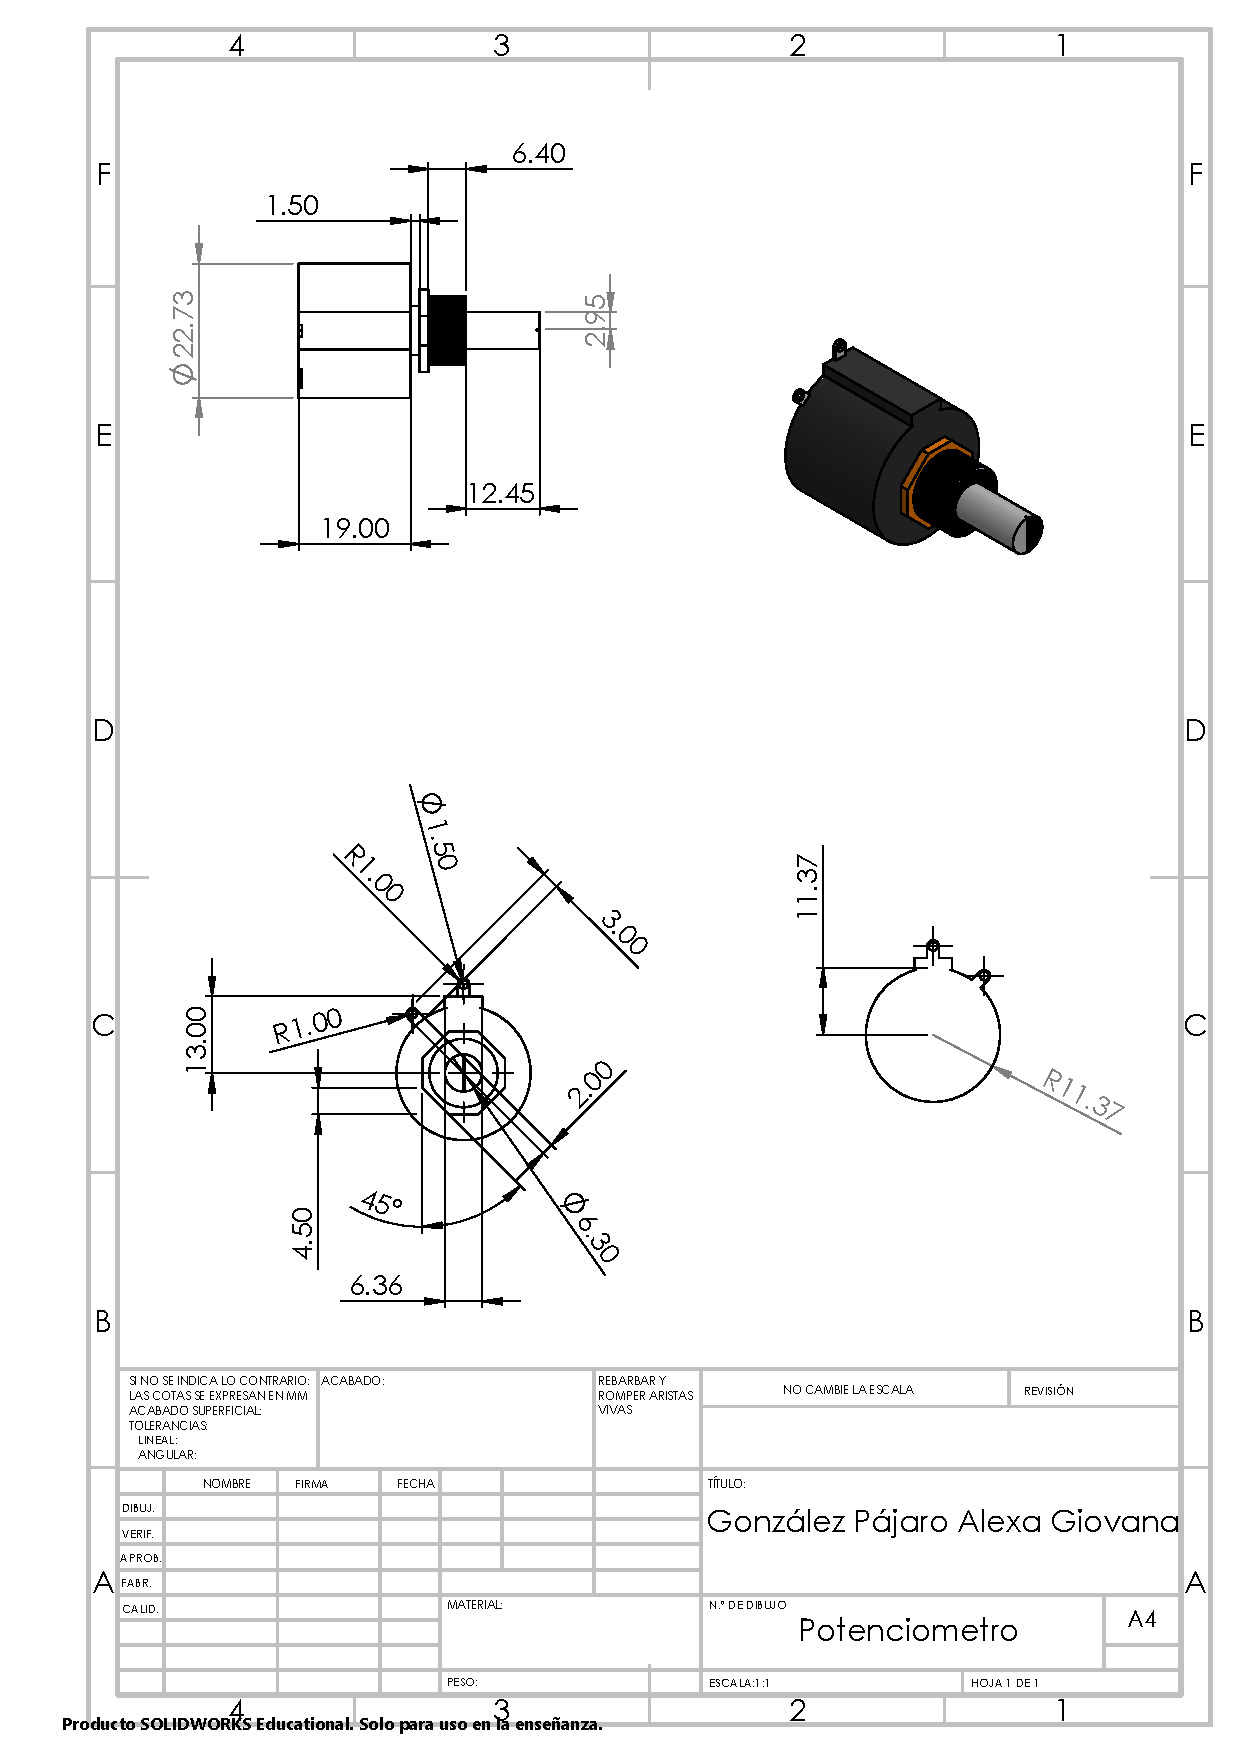
\includepdf[pages=-]{14/img/PlanoPotenciometro.PDF}
    %
    \centering{\section[\appendixautorefname{}]{Apéndice}}\label{anexo:PlanoResistencia}
    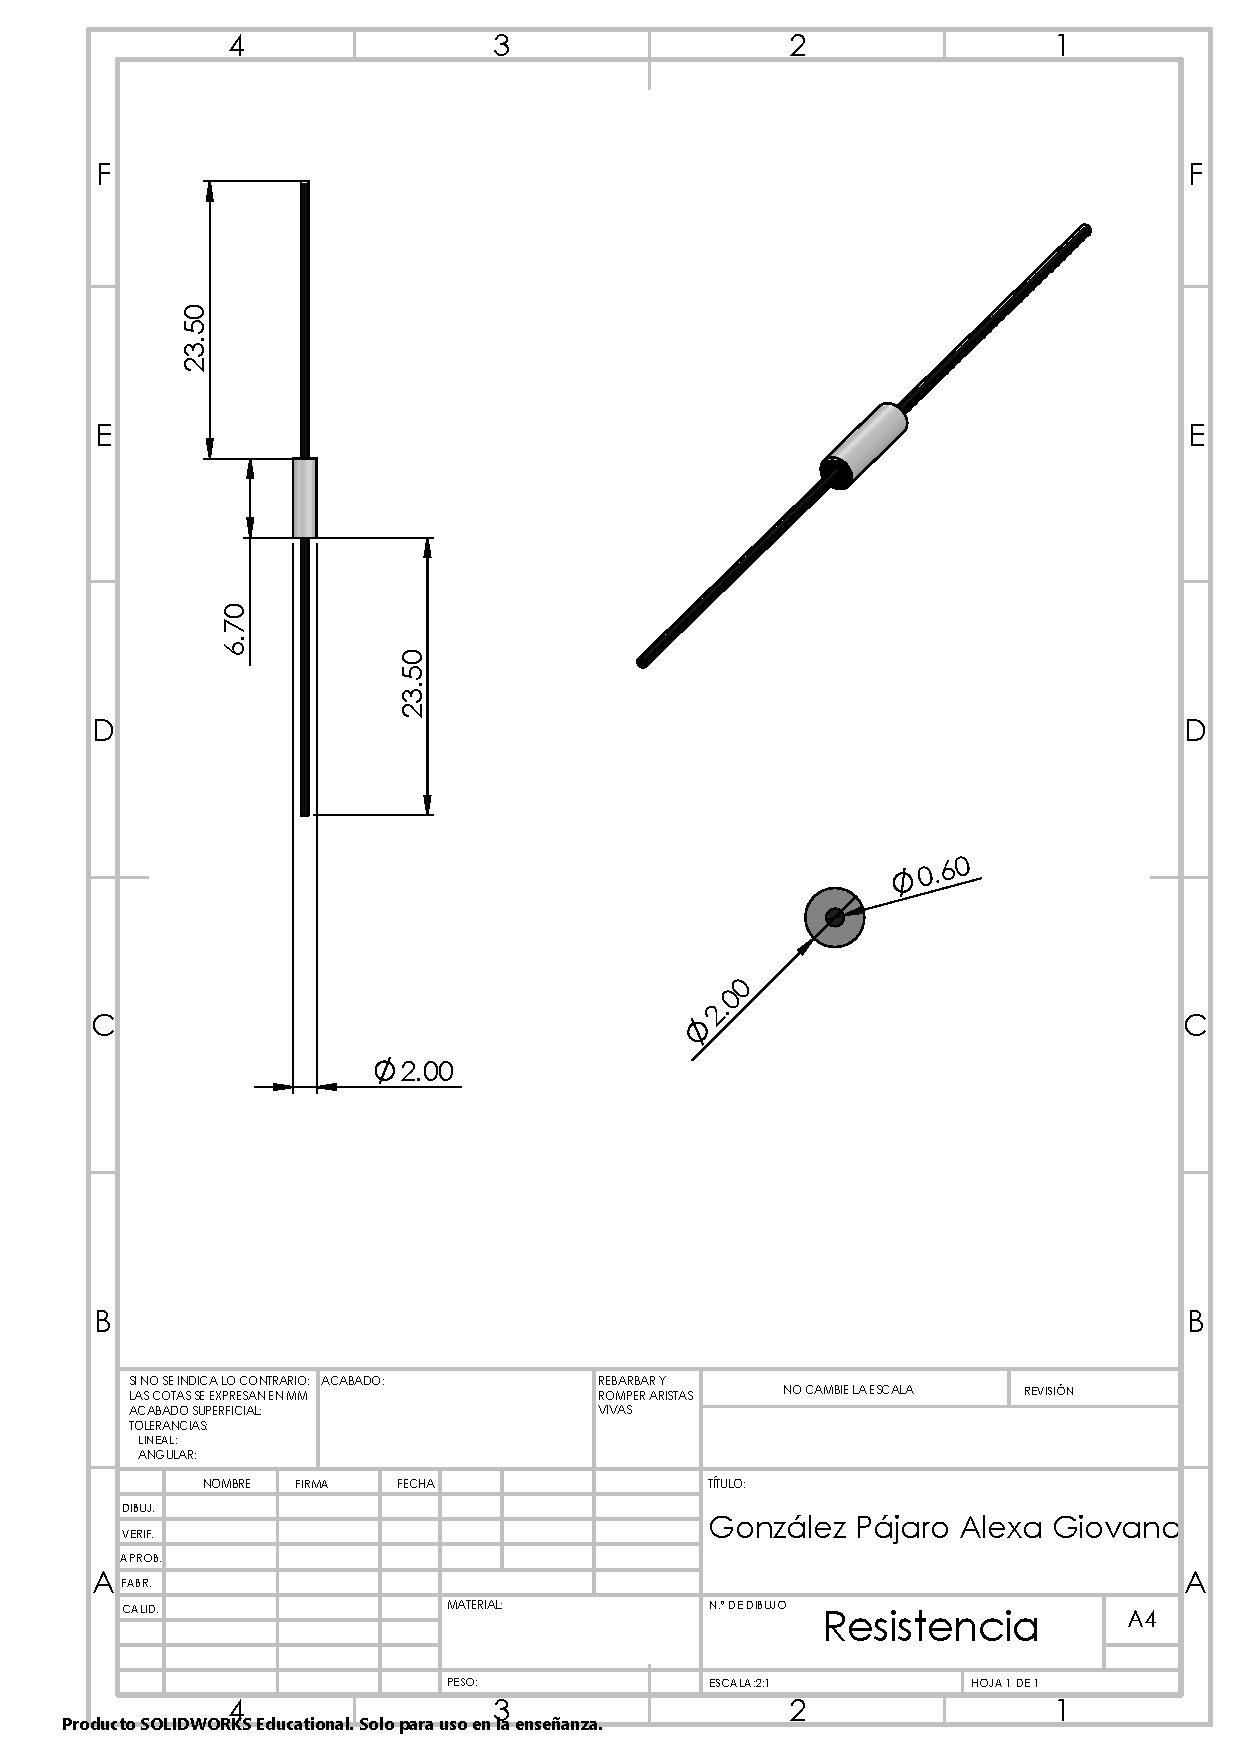
\includepdf[pages=-]{14/img/PlanoResistencia.pdf}
    %%%%%%%%%%%%%%%%%%%%%%%%%%%%%%%%%%%%%%%%